\documentclass[twoside]{article}

\usepackage[accepted]{aistats2026}

\usepackage[utf8]{inputenc}
\usepackage[T1]{fontenc}
\usepackage{natbib}
\usepackage{hyperref}
\usepackage{url}
\usepackage{booktabs}
\usepackage{multirow}   % tables/benchmark_gap.tex uses \multirow
\usepackage{amsmath, amssymb, amsthm, amsfonts, mathtools}
\usepackage{algorithm}
\usepackage{algorithmic}
\usepackage{graphicx}
\usepackage{adjustbox}  % max width=... shrinks oversized tables to fit (never enlarges)
\usepackage{xcolor}
\usepackage{enumitem}
\usepackage{tikz}
\usetikzlibrary{arrows.meta, positioning, fit, backgrounds, shapes}

% Relax float-placement fractions so two full-width floats may share a page top;
% without this the related-work table strands alone on a near-empty page.
\renewcommand{\dbltopfraction}{0.9}
\renewcommand{\topfraction}{0.9}
\renewcommand{\textfraction}{0.07}
\setcounter{dbltopnumber}{3}

% ---- shared DAG-figure styles (Fig. 1 + the appendix C-DAG figures) ----------
% Okabe-Ito colorblind-safe palette; latent confounding is drawn dash-dotted
% (one style for intra- and cross-cluster: the cluster boxes already show which
% pairs are inside a cluster).
\definecolor{okorange}{HTML}{E69F00}
\definecolor{okblue}{HTML}{56B4E9}
\definecolor{okpurple}{HTML}{CC79A7}
\tikzset{
  obsnode/.style={circle,draw=black!75,minimum size=6.5mm,inner sep=1pt,font=\small},
  mannode/.style={obsnode,fill=okorange!45},
  tgtnode/.style={obsnode,fill=okblue!45},
  clbox/.style={draw=black!55,dashed,rounded corners,inner sep=3.2mm},
  diredge/.style={->,>=Stealth,semithick,black!80},
  bicross/.style={<->,>=Stealth,okpurple,dashdotted,semithick},
  biintra/.style={bicross},% legacy alias kept for generated figures
}

\newtheorem{theorem}{Theorem}
\newtheorem{definition}{Definition}
\newtheorem{proposition}{Proposition}
\newtheorem{corollary}{Corollary}
\newtheorem{remark}{Remark}
\newtheorem{assumption}{Assumption}

\newcommand{\R}{\mathbb{R}}
\newcommand{\E}{\mathbb{E}}
% NB: named \doo, NOT \do -- LaTeX's list machinery (\@for etc.) redefines \do
% at runtime, which silently deleted every "do" from the rendered math.
\newcommand{\doo}{\mathrm{do}}
\newcommand{\Pa}{\mathrm{Pa}}
\newcommand{\QCBO}{\textsc{QCBO}}
\newcommand{\HQCBO}{\textsc{HQCBO}}
\newcommand{\QMCBO}{\textsc{QMCBO}}
\newcommand{\CBO}{\textsc{CBO}}
\newcommand{\BO}{\textsc{BO}}
\newcommand{\CEO}{\textsc{CEO}}
\newcommand{\Gg}{\mathcal{G}}
\newcommand{\Gq}{\mathcal{G}^{\Pi}}
\newcommand{\ES}{\mathbf{ES}}
\newcommand{\ESpi}{\mathbf{ES}^{\Pi}}
\newcommand{\TODO}[1]{{\color{red!75!black}\bfseries [TODO: #1]}}

% =============================================================================
\begin{document}

\runningtitle{Coarsening Confers Robustness in Causal Bayesian Optimization}
\runningauthor{Anonymous}

\twocolumn[
\aistatstitle{Coarsening Confers Robustness: \\ Causal Bayesian Optimization under DAG Misspecification}
\aistatsauthor{Anonymous}
\aistatsaddress{Anonymous}
]

% =============================================================================
\begin{abstract}
Causal Bayesian optimization (\CBO{}) uses a causal graph to build informative
priors and prune the space of candidate interventions --- but requires the
entire DAG to be specified correctly, and a recent survey names robustness to
structural misspecification a central open problem
\citep{anonymous2026cbobench}. We propose coarsening as an input
contract: the practitioner supplies only a partition of the manipulable
variables and the cluster-level (quotient) graph, and we prove that any
optimizer whose graph-dependent components factor through this quotient is
invariant --- exploration sets, priors, surrogates, the entire trajectory ---
to every misspecification confined within a cluster. We instantiate the
contract twice: \QCBO{}, arm-based quotient \CBO{} with complete
identification on the C-DAG; and \QMCBO{}, which coarsens model-based
\CBO{}'s mechanism factorization. Both are byte-for-byte invariant under
within-cluster edge errors that measurably shift their full-DAG counterparts,
and coarsening concentrates the intervention budget. The price is resolution:
when the optimum splits a cluster, a fixed partition pays linear-in-$T$
regret, which plateau-triggered refinement down a declared hierarchy turns
into a bounded transient. The trade is intrinsic: sub-cluster interventions
are provably not identifiable from quotient-level inputs alone --- resolution
must be bought with exposure.
\end{abstract}

% =============================================================================
\section{Introduction}
\label{sec:intro}

Causal Bayesian optimization \citep{aglietti2020causal} unifies two ideas: when the variable $Y$ we wish to optimize sits inside a causal system, the right search space is the space of interventions $\doo(\mathbf{X}_s=\mathbf{x}_s)$, and observational data plus the causal graph yield informative priors over the interventional response surfaces. The catch is the input requirement: \CBO{} and its descendants \citep{aglietti2021dynamic,aglietti2023constrained,sussex2023model} assume the full DAG is specified correctly, and the survey of \citet{anonymous2026cbobench} lists robustness to structural error among the field's open problems. Our thesis is that this fragility is best addressed by committing to less structure of a more reliable kind.

\paragraph{A wrong edge is costly.}
The assumed graph enters a \CBO{} algorithm only through its derived causal-effect estimators, and it corrupts them in two ways: it biases the do-calculus prior, and it can change the search set itself, possibly removing the candidate that contains the optimum. Either way the damage is a functional of the wrong edge: an estimator that cannot see an edge cannot be damaged by it. Remark~\ref{rem:taxonomy} makes the dichotomy precise, and the evaluation of \S\ref{sec:exp} is organized around it.

\paragraph{Coarser commitments decide less, so less can be wrong.}
A cluster-level structural belief encodes strictly fewer decisions than a
full DAG: one aggregate judgement between two groups of variables stands in
for a bundle of edge-level judgements the modeler is never asked to make.
Both ends of this spectrum are served --- full-DAG \CBO{} at one end, methods
that learn structure online at heavy per-trial cost at the other
\citep{mukherjee2024gacbo,branchini2023ceo}. The practical middle ---
reliable cluster-level structure --- has a developed identification theory
\citep{anand2023cdag,ferreira2025cdmg,wahl2024foundations} but, to our
knowledge, no optimization method.

\paragraph{Quotient \CBO{}.} \QCBO{} fills this gap. The practitioner supplies a partition $\Pi$ of the manipulable variables and the C-DAG $\Gq$ over its clusters (when a fine-grained hypothesis graph is available, $\Gq$ is its quotient, with bidirected edges absorbing latent confounding; \citealp{lee2019latent}). \QCBO{} explores cluster-level interventions whose effects are identifiable from $\Gq$, with identified cluster-level do-calculus estimates as GP prior means. This input never looks inside a cluster: an edge error confined to a cluster cannot even be represented, let alone affect the optimizer.

\paragraph{Contributions.}
\begin{itemize}[leftmargin=1.2em,itemsep=1pt,topsep=2pt]
  \item \textbf{Robustness as an input contract.} Quotient invariance is \emph{method-agnostic} (Theorem~\ref{thm:contract}): any optimizer whose graph-dependent components factor through $(\Pi,\Gq)$ is invariant to arbitrary within-cluster edge errors. We instantiate the contract arm-based (\QCBO{}, \S\ref{sec:method}) and model-based (\QMCBO{}, \S\ref{sec:qmcbo}).
  \item \textbf{Sample efficiency.} Coarsening concentrates a fixed budget on fewer identifiable cluster-level arms; Prop.~\ref{prop:price} characterizes its cost.
\end{itemize}

% =============================================================================
\section{Background}
\label{sec:background}

A structural causal model $\mathcal{M}=\langle\mathbf{U},\mathbf{V},F, P(\mathbf{U})\rangle$ induces a distribution over observables $\mathbf{V}$ and, for any $\mathbf{X}_s\subseteq\mathbf{V}$, interventional distributions $P(\cdot\mid\doo(\mathbf{X}_s=\mathbf{x}_s))$ obtained by replacing the mechanisms of $\mathbf{X}_s$ with constants \citep{pearl2009causality}. The induced graph $\Gg$ has a directed edge per functional argument and a bidirected edge per shared latent; projecting out latents yields an ADMG over $\mathbf{V}$ \citep{lee2019latent}. 

\paragraph{Causal Bayesian optimization.}
Given manipulable variables $\mathbf{X}\subseteq\mathbf{V}$ and target $Y$,
\CBO{} \citep{aglietti2020causal} solves
\begin{equation}
  \label{eq:cbo_obj}
  (\mathbf{X}_s^\star,\mathbf{x}_s^\star) =
  \arg\min_{\substack{\mathbf{X}_s\in\ES\\ \mathbf{x}_s\in D(\mathbf{X}_s)}} \E\!\left[Y\mid\doo(\mathbf{X}_s=\mathbf{x}_s)\right],
\end{equation}
where $D(\mathbf{X}_s)$ is the interventional domain of $\mathbf{X}_s$, maintaining one GP per candidate intervention set $\mathbf{X}_s$ in an exploration set $\ES$, with prior mean given by the do-calculus estimate of $\E[Y\mid\doo(\mathbf{X}_s=\mathbf{x}_s)]$ from observational data and the assumed graph, and selecting $(\mathbf{X}_s,\mathbf{x}_s)$ by expected improvement \citep{garnett2023bayesian}. Each candidate is itself a continuous BO sub-problem over $\mathbf{x}_s$. The exploration set is pruned structurally (MIS/POMIS; \citealp{lee2018structural}); both the pruning and the priors are functions of the assumed graph, which is where misspecification enters.

\paragraph{Coarsening and C-DAGs.}
\begin{definition}[Coarsening~\citep{madaleno2026coarsening}]
\label{def:coarsening}
Given a DAG $\Gg$ on $\mathbf{V}$, a partition $\Pi=\{C_1,\ldots,C_K\}$ of $\mathbf{V}$ induces the surjection $\chi:\mathbf{V}\to\Pi$ mapping each vertex to its cluster, and the quotient graph $\Gq$ with vertex set $\Pi$ and edge set $\{\chi(V_i)\to\chi(V_j) \mid V_i\to V_j\in\Gg,\ \chi(V_i)\neq\chi(V_j)\}$. If $\Gq$ is acyclic, it is a \textbf{coarsening} of $\Gg$ and $\Pi$ is valid. 
\end{definition}
For ADMGs the quotient additionally carries $C_k\leftrightarrow C_\ell$ iff some $V_i\in C_k,V_j\in C_\ell$ share a bidirected edge. The result is a C-DAG in the sense of \citet{anand2023cdag}: do-calculus on it is sound and complete for the class of fine graphs that quotient to it. Markov properties transfer to the cluster level; faithfulness does not \citep{wahl2024foundations}.

% =============================================================================
\section{Quotient \CBO{} (\QCBO{})}
\label{sec:method}

\subsection{Setup}
\label{sec:setup}
\QCBO{} uses only cluster-level structure: a partition $\Pi$ of the manipulable variables $\mathbf{X}$ and a C-DAG $\Gq$ over its clusters and the singleton nodes ($Y$ and every non-manipulable observable stay singletons; mixing manipulable and non-manipulable variables in one cluster is disallowed, since intervening on a cluster --- jointly setting all its members, $\doo(C_k=\mathbf{c}_k)$ --- must be executable). When the practitioner instead holds a fine-grained hypothesis graph $\Gg$, $\Gq$ is its quotient after projecting out hidden confounders \citep{lee2019latent}; \QCBO{} itself never requires the fine graph. The candidate exploration set contains all unions of at most $m$ clusters:
\begin{equation}
  \label{eq:ccbo_exploration}
  \ESpi_{0} = \Bigl\{\,\bigcup_{C_k\in\mathcal{S}}C_k \;\Big|\;
  \emptyset\neq\mathcal{S}\subseteq\Pi,\;|\mathcal{S}|\leq m\,\Bigr\}.
\end{equation}

Merging manipulable variables coarsens the action space: \QCBO{} can only set a cluster jointly, never a strict subset of it --- the mechanism behind both the robustness (\S\ref{sec:theory}) and the price (Prop.~\ref{prop:price}) of coarsening. Algorithm~\ref{alg:ccbo} (App.~\ref{app:repro}) summarizes the loop.

\subsection{Identifiable exploration set and the two-tier prior}
\label{sec:causal_prior}
For each candidate $\mathbf{X}_s\in\ESpi_0$ we pose the cluster-level query $P(Y\mid\doo(\mathbf{X}_s))$ on $\Gq$ and run the complete ID algorithm of \citet{shpitser2006identification} (via \texttt{ananke}; \citealp{lee2023ananke}). Following the arm-pruning tradition of structural causal bandits \citep{lee2018structural}, \QCBO{} \emph{commits to its structural beliefs}: the exploration set keeps exactly the candidates whose effect is identifiable from $\Gq$,
\begin{equation}
  \label{eq:es_gate}
  \ESpi = \{\,\mathbf{X}_s\in\ESpi_0 \,:\, P(Y\mid\doo(\mathbf{X}_s))\text{ id.\ from }\Gq\,\}.
\end{equation}
This restriction is exact (ID is complete on the C-DAG, and identification from $\Gq$ is sound for every fine graph in its class \citealp{anand2023cdag}).

For $\mathbf{X}_s\in\ESpi$, the GP prior mean is constructed in two steps: the identified formula is instantiated as a pipeline of GP-based plug-ins (backdoor $\to$ front-door $\to$ $g$-computation) on the bidirected-edge expansion of $\Gq$, falling back to the observational mean on the queries the sound-but-incomplete pipeline cannot instantiate:
\begin{equation}
  \label{eq:two_tier_prior}
  m_s(\mathbf{x}_s) = \begin{cases}
    \hat{\E}[Y\mid\doo(\mathbf{X}_s=\mathbf{x}_s)] & \text{cascade succeeds,}\\
    \bar{Y}_{\mathrm{obs}} & \text{otherwise.}
  \end{cases}
\end{equation}
Because clusters are manipulable-only and interventions assign full clusters, the cluster-level formulas expand exactly into fine-grained regressions on observational data.

\begin{assumption}[Valid C-DAG]
\label{ass:valid}
The directed part of $\Gq$ is acyclic. This constrains only inter cluster structure (intra-cluster acyclicity can even be relaxed; \citealp{madaleno2026cycles}), coincides with validity of the coarsening (Def.~\ref{def:coarsening}) when $\Gq$ is a quotient, and is checkable directly on the cluster-level object.
\end{assumption}

\begin{assumption}[Estimator-completeness boundary]
\label{ass:id_scheme}
The ID test (Eq.~\ref{eq:es_gate}) is complete; the estimator cascade behind Eq.~\eqref{eq:two_tier_prior} is sound but not complete, and identifiable queries it misses receive the uninformative tier (in \S\ref{sec:exp} this set is empty).
\end{assumption}

% =============================================================================
\section{What coarsening buys}
\label{sec:theory}
Throughout, $\Pi,\Pi'$ are manipulable-only partitions; $\Pi_\bot$ is the finest (all-singleton) partition, the bottom of the partition refinement lattice \citep{madaleno2026coarsening}; $\Pi'\preceq\Pi$ ($\Pi'$ refines $\Pi$) iff every cluster of $\Pi'$ is contained in a cluster of $\Pi$. Props.~\ref{prop:refinement_validity}--\ref{prop:price} relate quotients of a common underlying graph; \QCBO{} itself consumes only $\Gq$ (Assumption~\ref{ass:valid}).

\begin{proposition}[Identity recovery]
\label{prop:identity}
Under $\Pi=\Pi_\bot$, $\Gq=\Gg^{*}$ and $\ESpi_0$ is the set of all subsets of $\mathbf{X}$ of size at most $m$; \QCBO{} reduces to full-DAG \CBO{}, with the exploration set restricted to the identifiable subsets.
\end{proposition}

\begin{theorem}[Quotient invariance is method-agnostic]
\label{thm:contract}
Let $\mathcal{A}$ be any causal Bayesian optimizer each of whose graph-dependent components --- search space, identification formulas, priors, surrogate architecture, and selection rules --- depends on the structural hypothesis $\Gg$ only through the pair $(\Pi, \Gq)$, where $\Gq$ is the quotient of $\Gg$'s latent projection under a valid $\Pi$. Then for any two acyclic hypotheses $\Gg,\Gg'$ with $(\Gg')^{\Pi}=\Gq$, and the same data, seeds, and hyperparameters, $\mathcal{A}$ produces identical trajectories under $\Gg$ and $\Gg'$. In particular, this holds for every edit (insertion, deletion, or reversal of directed or bidirected edges) confined within a single cluster, and for inter-cluster edits that are redundant in the quotient. (Proof: App.~\ref{app:proofs})
\end{theorem}

\begin{proposition}[Invariance to intra-cluster misspecification]
\label{prop:invariance}
Let $\Pi$ be valid for $\Gg$ and let acyclic $\Gg'$ differ from $\Gg$ by any set of insertions, deletions, or reversals of (directed or bidirected) edges whose endpoints lie within a single cluster of $\Pi$. Then $(\Gg')^{\Pi}=\Gq$, and --- since all of \QCBO{}'s graph-dependent components are functions of $(\Pi,\Gq)$ --- Theorem~\ref{thm:contract} applies: the exploration set, every prior, and, given the same data and seeds, the entire trajectory are identical under $\Gg$ and $\Gg'$. The conclusion holds for any acyclic $\Gg'$ with $(\Gg')^{\Pi}=\Gq$, i.e.\ every quotient-invisible perturbation.
\end{proposition}

\begin{remark}[Exact scope]
\label{rem:structural_robustness}
Prop.~\ref{prop:invariance} states that \QCBO{} cannot represent an intra-cluster hypothesis, so no intra-cluster mistake can affect it. The precise condition is that the perturbed edge be invisible in the quotient: intra-cluster edges, and inter-cluster edges that are redundant (e.g a parallel edge from another cluster member). A quotient-visible edge is not protected: \S\ref{sec:exp-scope} shows the same bow misspecification, with endpoints in different clusters, removing a cluster-level arm from the identifiable exploration set.
\end{remark}

\begin{remark}[How a wrong graph enters the algorithm]
\label{rem:taxonomy}
A wrong assumed graph reaches any causal Bayesian optimizer through its derived causal-effect estimators, in two ways. \emph{Prior bias:} for any arm whose identifying estimand references the misspecified edge, the do-calculus prior mean is biased --- even though the \emph{true} effect is unchanged --- and expected improvement wastes evaluations until interventional data correct it, a convergence cost paid in GAP/PA-GAP. \emph{Search-set change:} the exploration set is itself derived from the graph --- (PO)MIS pruning in full-DAG \CBO{} \citep{lee2018structural,aglietti2020causal}, the identifiability gate (Eq.~\ref{eq:es_gate}) in \QCBO{} --- so the wrong graph can flip a verdict and remove an arm (or admit a spurious one), a cost in sample efficiency or, under a budget cap, in reachable optimum. Coarsening closes both channels whenever the misspecified edges are quotient-invisible (Prop.~\ref{prop:invariance}): the quotient never references the edge, so no estimator it forms is biased and no verdict it makes is flipped.
\end{remark}

\begin{proposition}[Validity is not refinement-monotone]
\label{prop:refinement_validity}
There exist a valid $\Pi$ and a refinement $\Pi'\preceq\Pi$ whose quotient is cyclic; validity must be re-verified after each refinement (it remains decidable from cluster-level structure alone).
\end{proposition}

\begin{proposition}[Monotonicity under valid refinement]
\label{prop:refinement}
Let $\Pi'\preceq\Pi$ with both valid and $m=\infty$. Then (i) $\ESpi_0\subseteq\ES^{\Pi'}_{0}$; (ii) every $\mathbf{X}_s\in\ESpi$ is also in $\ES^{\Pi'}$, with the same identification functional.
\end{proposition}

\begin{proposition}[Price of coarsening]
\label{prop:price}
Let $\mu^\star(\mathbf{X}_s)=\min_{\mathbf{x}_s\in D(\mathbf{X}_s)} \E[Y\mid\doo(\mathbf{X}_s=\mathbf{x}_s)]$ and $V(\Pi)=\min_{\mathbf{X}_s\in\ESpi_0}\mu^\star(\mathbf{X}_s)$, with $m=\infty$. For any valid $\Pi'\preceq\Pi$, $V(\Pi_\bot)\le V(\Pi')\le V(\Pi)$, and $V(\Pi)=V(\Pi_\bot)$ iff some optimizer $\mathbf{X}_s^\star$ of Eq.~\eqref{eq:cbo_obj} is a union of $\Pi$-clusters.
\end{proposition}

\subsection{Refining the partition: Hierarchical-\QCBO{}}
\label{sec:refine}
When no optimizer is a union of $\Pi$-clusters, a fixed-partition run pays $V(\Pi)-y^\star>0$ \emph{forever}: $R_T/T\to V(\Pi)-y^\star$. This failure is different from full-DAG \CBO{}'s --- a \emph{missing arm}, which no amount of data can restore, versus a biased prior that interventional data eventually override. Refinement converts the uncorrectable kind back into the correctable kind by treating $\Pi$ as a starting resolution.

The practitioner may declare a \emph{hierarchy} $H$: per cluster, an optional sub-partition (default: singletons); no new graph is supplied. \HQCBO{} runs Algorithm~\ref{alg:ccbo} at $\Pi$ and, when the incumbent improves by less than $\delta$ over $k$ trials ($k{=}5$, $\delta{=}10^{-3}$, tuned once and fixed), splits the incumbent arm's clusters via $H$. Validity is re-checked (Prop.~\ref{prop:refinement_validity}); an invalid split is \emph{refused}. On acceptance, the exploration set is rebuilt and unlocked with every explored arm, data are carried over keyed by arm (Prop.~\ref{prop:refinement}), and only new arms receive the standard $n_0$ initialization points (App.~\ref{app:refine}); we evaluate a single refinement step.

\begin{remark}[Phase-scoped invariance]
\label{rem:phase_invariance}
Any misspecification that is quotient-invisible at \emph{every} visited partition --- in particular, inside a cluster that is never split --- leaves the entire refine trajectory unchanged, including the trigger time and the refinement decision (per phase this is Prop.~\ref{prop:invariance}; the trigger is a function of the trajectory and $H$ alone). Refining a cluster \emph{spends} its invariance: edits inside a split cluster are exposed after the trigger.
\end{remark}

\begin{remark}[The price becomes a transient]
\label{rem:regret}
If the exploration set at some visited partition contains an optimal arm and the base optimizer is consistent on a finite arm set, the incumbent converges to $y^\star$ and $R_T \le t_r\,r_0 + o(T)$ ($t_r$ the trigger time, $r_0$ the initial regret) --- versus $\Theta(T)$ for the fixed partition. The trigger never observes $y^\star$, so it also fires on lossless partitions; there refinement costs only the new arms' initialization and, empirically, a small refinement price (\S\ref{sec:exp-partition}).
\end{remark}

% =============================================================================
\section{Model-based \QCBO{}}
\label{sec:qmcbo}
Model-based \CBO{} (MCBO; \citealp{sussex2023model}) couples the surrogate to the graph more tightly than \CBO{}: it fits one GP per \emph{mechanism} and evaluates interventions by composing these GPs along the DAG. The graph is the surrogate's \emph{architecture}, a wrong intra-cluster edge corrupts the factorization every prediction flows through.

\textbf{Construction (\QMCBO{}).} Coarsen the factorization: one \emph{joint} mechanism per cluster, $P(\mathbf{X}_C \mid \mathbf{X}_{\mathrm{pa}(C)})$, modeled as a multi-output GP (ICM task kernel; singleton clusters reduce to MCBO's per-node GPs), composed along the C-DAG with joint within-cluster sampling; do() targets are lifted to whole-cluster patterns. 

\begin{corollary}[\QMCBO{} inherits the contract]
\label{cor:qmcbo_invariance}
Every graph-dependent component of \QMCBO{} is a function of $(\Pi,\Gq)$, so Theorem~\ref{thm:contract} applies: quotient-invisible edits leave its entire trajectory unchanged. Moreover, (i) at $\Pi=\Pi_\bot$, \QMCBO{} is exactly MCBO; and (ii) \QMCBO{}'s arm space equals \QCBO{}-coarse's, so Prop.~\ref{prop:price} applies: on a lossy partition, no amount of data recovers $y^\star$.
\end{corollary}

\begin{proposition}[Soundness of cluster mechanisms]
\label{prop:qsound}
Assume causal sufficiency and a valid $\Pi$. For every union-of-clusters intervention, the cluster-level truncated factorization --- the true joint cluster mechanisms composed along the C-DAG with intervened clusters together --- equals $P(\mathbf{V}\mid\doo(\mathbf{x}_S))$. (Proof: App.~\ref{app:proofs}.) The per-coordinate variant is its approximation, exact when clusters contain no intra-cluster edges; we ablate the two in \S\ref{sec:exp}.
\end{proposition}

\begin{proposition}[Exposure: sub-cluster interventions are not identifiable
from cluster mechanisms]
\label{prop:qexposure}
There exist SCMs $M_1, M_2$, causally sufficient and valid for the same $\Pi$, with identical joint cluster mechanisms and identical interventional distributions for every union-of-clusters intervention, yet $P^{M_1}(Y\mid\doo(\mathbf{x}_A)) \neq P^{M_2}(Y\mid\doo(\mathbf{x}_A))$ for a strict subset $A\subsetneq C$ of some cluster. (Proof: App.~\ref{app:proofs}.) Consequently \emph{no} quotient-respecting method --- arm-based or model-based --- can evaluate sub-cluster arms from its inputs alone: \S\ref{sec:refine} is a property of the quotient contract itself, not of our refinement procedure.
\end{proposition}

% =============================================================================
\section{Experiments}
\label{sec:exp}

\subsection{Setup: head-to-head under misspecification}
\label{sec:exp-setup}
\paragraph{ClusterBench10.}
We construct an SCM (Fig.~\ref{fig:clusterbench10}) with ten observables: manipulable $X_1,\dots,X_5$, mediators $M_1,M_2,M_3,M_4$, target $Y$, latent confounders $U_{12}\!\to\!\{X_1,X_2\}$ (intra-cluster) and $U_{15}\!\to\!\{X_1,X_5\}$ (cross-cluster); the coarse partition is $C_1=\{X_1,X_2,X_3\}$, $C_2=\{X_4,X_5\}$. Coefficients are chosen so that (i) $\doo(X_1)$ is the strongest \emph{singleton} intervention, (ii) the global optimum is $\doo(C_1)$ --- a union of clusters, so the partition is \emph{lossless} and any robustness gap is not confounded by a price of coarsening --- and (iii) $\mathrm{corr}(X_1,X_2)\approx 0.70$, (full specification and oracle checks in App.~\ref{app:scm}).

\begin{figure*}[t]\centering
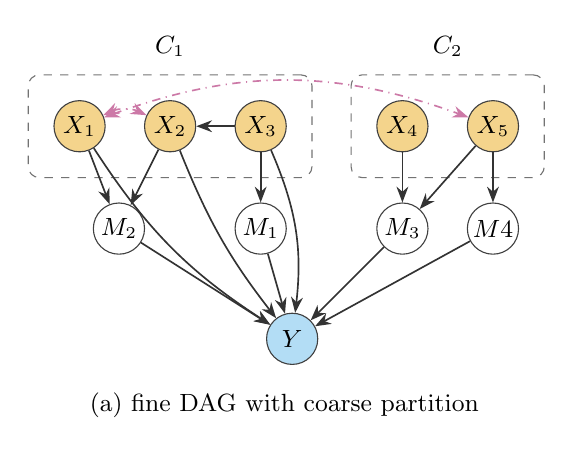
\begin{tikzpicture}
  % ---- (a) fine DAG with the coarse partition ----
  \node[mannode] (X1) at (0,2.4) {$X_1$};
  \node[mannode] (X2) at (1.15,2.4) {$X_2$};
  \node[mannode] (X3) at (2.3,2.4) {$X_3$};
  \node[mannode] (X4) at (4.1,2.4) {$X_4$};
  \node[mannode] (X5) at (5.25,2.4) {$X_5$};
  \node[obsnode] (M2) at (0.5,1.1) {$M_2$};
  \node[obsnode] (M1) at (2.3,1.1) {$M_1$};
  \node[obsnode] (M3) at (4.1,1.1) {$M_3$};
  \node[obsnode] (M4)  at (5.25,1.1) {$M4$};
  \node[tgtnode] (Y)  at (2.7,-0.3) {$Y$};
  \draw[diredge] (X3) -- (X2);
  \draw[diredge] (X1) -- (M2); \draw[diredge] (X2) -- (M2);
  \draw[diredge] (X3) -- (M1);
  \draw[diredge] (X4) -- (M3); \draw[diredge] (X5) -- (M3);
  \draw[diredge] (X5) -- (M4);
  % X1/X2 bend west and X3 bends east so none of them clips M1.
  \draw[diredge] (X1) to[bend right=12] (Y);
  \draw[diredge] (X2) to[bend right=8] (Y);
  \draw[diredge] (X3) to[bend left=15] (Y);
  \draw[diredge] (M1) -- (Y); \draw[diredge] (M2) -- (Y);
  \draw[diredge] (M3) -- (Y); \draw[diredge] (M4) -- (Y);
  % Latent confounding: the intra-C1 arc stays inside the cluster box; the
  % cross-cluster arc bends lower so it cannot collide with the cluster labels.
  \draw[bicross] (X1) to[bend left=25] (X2);
  \draw[bicross] (X1) to[bend left=20] (X5);
  \begin{scope}[on background layer]
    \node[clbox,fit=(X1)(X2)(X3),label={[label distance=1mm]above:{\small$C_1$}}] {};
    \node[clbox,fit=(X4)(X5),label={[label distance=1mm]above:{\small$C_2$}}] {};
  \end{scope}
  \node at (2.6,-1.15) {\small (a) fine DAG with coarse partition};
\end{tikzpicture}
\hspace{1.2cm}
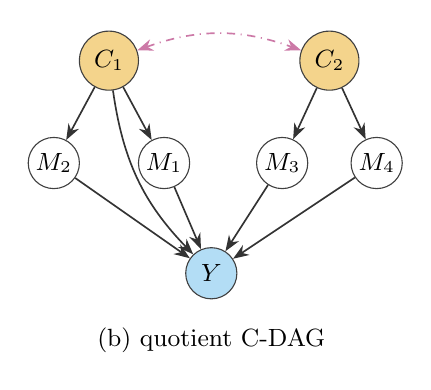
\begin{tikzpicture}
  % ---- (b) quotient C-DAG; clusters sit centred over their mediators so the
  %      quotient map from (a) is visually immediate ----
  \node[mannode,minimum size=7.5mm] (C1) at (0.6,2.4) {$C_1$};
  \node[mannode,minimum size=7.5mm] (C2) at (3.4,2.4) {$C_2$};
  \node[obsnode] (M2) at (-0.1,1.1) {$M_2$};
  \node[obsnode] (M1) at (1.3,1.1) {$M_1$};
  \node[obsnode] (M3) at (2.8,1.1) {$M_3$};
  \node[obsnode] (M4)  at (4.0,1.1) {$M_4$};
  \node[tgtnode] (Y)  at (1.9,-0.3) {$Y$};
  \draw[diredge] (C1) -- (M1); \draw[diredge] (C1) -- (M2);
  \draw[diredge] (C1) to[bend right=18] (Y);
  \draw[diredge] (C2) -- (M3); \draw[diredge] (C2) -- (M4);
  \draw[diredge] (M1) -- (Y); \draw[diredge] (M2) -- (Y);
  \draw[diredge] (M3) -- (Y); \draw[diredge] (M4) -- (Y);
  \draw[bicross] (C1) to[bend left=20] (C2);
  \node at (1.9,-1.15) {\small (b) quotient C-DAG};
\end{tikzpicture}
\\[5pt]
{\scriptsize
  \tikz{\node[mannode,minimum size=3.6mm,font=\tiny] {};}\,manipulable\quad
  \tikz{\node[obsnode,minimum size=3.6mm,font=\tiny] {};}\,non-manipulable\quad
  \tikz{\node[tgtnode,minimum size=3.6mm,font=\tiny] {};}\,target\quad
  \tikz{\draw[diredge] (0,0) -- (0.5,0);}\,direct effect\quad
  \tikz{\draw[bicross] (0,0) -- (0.5,0);}\,confounding\quad
  \tikz{\draw[clbox,inner sep=0pt] (0,-0.07) rectangle (0.42,0.13);}\,cluster
}
\caption{\textbf{ClusterBench10.} In the quotient (b), the intra-cluster
confounding $X_1\!\leftrightarrow\!X_2$ disappears while the cross-cluster
$X_1\!\leftrightarrow\!X_5$ becomes $C_1\!\leftrightarrow\!C_2$. Hence the
\emph{intra} bow (adding $X_1\!\to\!X_2$) is invisible to the quotient,
whereas the \emph{inter} bow (adding $X_1\!\to\!X_5$) completes a
cluster-level bow, rendering $\doo(C_1)$ non-identifiable and removing it
from the coarse exploration set.}
\label{fig:clusterbench10}
\end{figure*}

\paragraph{Fixed-objective protocol.}
We hold fixed the true SCM, observational data, $y^\star$, seeds, and budget, and inject the misspecification only into the assumed structure each causal method reasons with, verifying that the injection leaves the objective byte-identical under every perturbation (App.~\ref{app:seam}).

\paragraph{Perturbations, methods, and metrics.}
We perturb the DAG by adding, deleting, or reversing edges, classified by whether their endpoints lie within a coarse cluster (\emph{intra}) or across clusters (\emph{inter}); the headline perturbation is a \emph{bow} --- a directed edge added on a latently-confounded pair, which renders the corresponding $\doo$-effect non-identifiable. The arms share one estimator, seeds, and initialization, differing only in the causal prior and the graph each identifies on (Table~\ref{tab:methods}). By Prop.~\ref{prop:identity}, \CBO{} \citep{aglietti2020causal} is exactly \QCBO{} at the finest partition, so the two rows coincide on \emph{every} graph; \QCBO{}-coarse runs the same algorithm on the quotient. \CEO{} \citep{branchini2023ceo} --- a  graph-uncertainty method --- runs through its authors' own stack under the same protocol (App.~\ref{app:seam}).

\begin{table}[t]\centering
  \caption{The experimental arms share seeds, budget, and evaluation oracle; they differ in the causal prior and the structure each reasons with. \CBO{}$\,\equiv\,$\QCBO{}-finest by Prop.~\ref{prop:identity} (listed once here; the equivalence holds on every graph). \CEO{} runs with a candidate-graph pool centered on the assumed DAG (App.~\ref{app:seam}).}
  \label{tab:methods}
  \small
  \adjustbox{max width=\linewidth}{\begin{tabular}{@{}llll@{}}
    \toprule
    \textbf{Method} & \textbf{Causal prior} & \textbf{Identifies on} & \textbf{Exploration set} \\
    \midrule
    \BO{} & none (zero mean) & --- & one joint arm (all vars) \\
    \CBO{}$\,\equiv\,$\QCBO{}-finest & do-calculus & full assumed DAG & (PO)MIS, full DAG \\
    \CEO{} & posterior-averaged & candidate DAG pool & subsets of $\mathbf{X}$ \\
    \textbf{\QCBO{}-coarse} & cluster do-calculus & quotient C-DAG & identifiable cluster unions \\
    \bottomrule
  \end{tabular}}
\end{table}
We score trajectories with GAP/PA-GAP protocol: GAP combines final improvement with how early it is attained, PA-GAP weights every trial's improvement by a linearly decaying factor, and in both higher is better in $[0,1]$; GAP@$k$ is GAP on the first $k$ trials. We report the paired-by-seed degradation $\Delta=\mathrm{metric}(\text{misspecified},s)-\mathrm{metric}(\text{correct},s)$, so per-seed noise cancels, alongside the simple regret $r_T=|y^{\mathrm{best}}_T-y^\star|$ and the cumulative regret $R_T=\sum_{t=1}^{T} r_t$ of the incumbent sequence.

\subsection{Coarsening guarantees an unchanged trajectory}
\label{sec:exp-headline}
We first fix the correct DAG (Table~\ref{tab:headline}): the causal methods exploit the observational prior to converge within a handful of interventions; non-causal \BO{}, learning the ten-dimensional response from scratch, is far slower and worst in absolute $Y$.

We then add the intra-cluster bow (add $X_1\!\to\!X_2$ on the $U_{12}$-confounded pair) with the objective held fixed. No method's final value is damaged --- the optimum $\doo(C_1)$ severs the bow for every method --- so the damage appears in convergence, where Remark~\ref{rem:taxonomy} predicts it. For \QCBO{}-coarse the bow lies inside $C_1$: its trajectory, GAP, and PA-GAP are unchanged ($\Delta=0$ exactly, Prop.~\ref{prop:invariance}). Full-DAG \CBO{}/\QCBO{}-finest deletes every arm the bow touches --- $\doo(X_1)$ and every superset leaving $X_2$ unintervened become unidentifiable --- so its GAP and PA-GAP shift (Table~\ref{tab:taxonomy}).

\paragraph{The same edit with the opposite sign.}
On this SCM the deletion even \emph{helps}: $\doo(X_1)$ is a "decoy", so removing it concentrates the budget on the larger arms containing the optimum (Fig.~\ref{fig:overlays}, App.~\ref{app:fulltables}). \textsc{ClusterBench10D} (App.~\ref{app:scm}) moves $Y$'s centers so the strongest singleton \emph{is} the global optimum while the coarse partition stays lossless: the identical bow now deletes the cheap optimal arm, and full-DAG \CBO{}'s cumulative regret rises $4.6\times$ (Table~\ref{tab:damage}, App.~\ref{app:scm}) --- a per-trial cost no data can repair, because the arm itself is gone. \QCBO{}-coarse is invariant on both variants. Deleting a decoy accelerates, deleting the optimal arm injures --- and which case one is in cannot be known without the very structure in doubt; Prop.~\ref{prop:invariance} removes the question for every quotient-invisible error.

\begin{table*}[t]\centering
  \caption{Sample efficiency on ClusterBench10 under the \emph{correct} DAG
  (mean$\pm$s.e., $10$ seeds, $T{=}100$; higher GAP/PA-GAP and lower
  $r_T$/$R_T$ are better).}
  \label{tab:headline}
  \adjustbox{max width=\linewidth}{\begin{tabular}{@{}lcccc@{}}
\toprule
\textbf{Method} & \textbf{Final $Y$} & \textbf{GAP@20} & \textbf{GAP@50} & \textbf{GAP@100} \\
\multicolumn{1}{c}{} & {\footnotesize $\downarrow$, $y^\star{=}0$} & \multicolumn{3}{c}{\footnotesize $\uparrow$ more sample-efficient} \\
\midrule
\BO & $1.386{\scriptstyle\,\pm\,}0.73$ & $0.52{\scriptstyle\,\pm\,}0.06$ & $0.67{\scriptstyle\,\pm\,}0.04$ & $0.78{\scriptstyle\,\pm\,}0.05$ \\
\CBO & $0.332{\scriptstyle\,\pm\,}0.11$ & $0.47{\scriptstyle\,\pm\,}0.06$ & $0.60{\scriptstyle\,\pm\,}0.08$ & $0.54{\scriptstyle\,\pm\,}0.05$ \\
\QCBO-finest & $0.245{\scriptstyle\,\pm\,}0.05$ & $0.44{\scriptstyle\,\pm\,}0.06$ & $0.50{\scriptstyle\,\pm\,}0.06$ & $0.60{\scriptstyle\,\pm\,}0.04$ \\
\textbf{\QCBO-coarse} & $0.128{\scriptstyle\,\pm\,}0.02$ & $0.73{\scriptstyle\,\pm\,}0.05$ & $0.89{\scriptstyle\,\pm\,}0.02$ & $0.77{\scriptstyle\,\pm\,}0.07$ \\
\bottomrule
\end{tabular}
}
\end{table*}

\subsection{Which misspecifications are protected?}
\label{sec:exp-scope}
A single controlled contrast delimits the scope: the \emph{same} operation --- adding a directed edge on a latently-confounded pair. The intra bow (add $X_1\!\to\!X_2$) leaves \QCBO{}-coarse unchanged. The inter bow (add $X_1\!\to\!X_5$, across $C_1,C_2$) forms a \emph{cluster-level} bow $C_1\to C_2$ with $C_1\leftrightarrow C_2$, making $\doo(C_1)$ --- the arm \QCBO{}-coarse relies on --- non-identifiable: the guarantee is lost and the trajectory moves off zero (Table~\ref{tab:taxonomy}). The other quotient-visible perturbation, the inter deletion, is unprotected yet unchanged on this SCM --- the deleted edge never enters the identification of an arm the optimizer uses --- so quotient-invisibility is \emph{sufficient} for invariance, not necessary. The field also contains the most realistic error of all: omitting the latent confounder $X_1\!\leftrightarrow\!X_2$ ($P_7$). No verdict flips --- the channel is pure prior bias --- yet the full-DAG trajectory reshuffles in a seed-dependent direction; the quotient discards intra-cluster bidirected edges, so \QCBO{}-coarse is again invariant. The severity dial (Fig.~\ref{fig:dial}, App.~\ref{app:fulltables}) confirms the pattern across the whole field: \QCBO{}-coarse stays at zero across the one-, two-, three-edit intra sweep and leaves zero only under the inter bow.

\begin{table*}[t]\centering
  \caption{Scope of the guarantee: paired $\Delta$GAP and $\Delta$PA-GAP@100 (misspecified $-$ correct; mean$\pm$s.e., $10$ seeds). \QCBO{}-coarse is exactly $\mathbf{0}$ (byte-identical, bold) on every quotient-invisible perturbation, as Prop.~\ref{prop:invariance} guarantees, and moves only under the inter bow. $0^{\dagger}$: \CEO{} coincides with its correct-graph run on $P_7$ only because its DAG pool cannot represent a confounder omission --- representational blindness, not a guarantee. \BO{} is $\equiv\!0$ by construction; full rows in App.~\ref{app:fulltables}.}
  \label{tab:taxonomy}
  \adjustbox{max width=\linewidth}{\begin{tabular}{@{}ll cc cc@{}}
\toprule
\textbf{Perturbation} & \textbf{Locus} & \multicolumn{2}{c}{\textbf{\QCBO-finest}} & \multicolumn{2}{c}{\textbf{\QCBO-coarse}} \\
\cmidrule(lr){3-4}\cmidrule(lr){5-6}
 & & $\Delta$GAP & $\Delta$PA-GAP & $\Delta$GAP & $\Delta$PA-GAP \\
\midrule
add $X_1\!\to\!X_2$ (bow) & intra & $+0.116{\scriptstyle\,\pm\,}0.043$ & $+0.122{\scriptstyle\,\pm\,}0.024$ & $\mathbf{0}$ & $\mathbf{0}$ \\
del $X_3\!\to\!X_2$ & intra & $+0.156{\scriptstyle\,\pm\,}0.039$ & $-0.004{\scriptstyle\,\pm\,}0.020$ & $\mathbf{0}$ & $\mathbf{0}$ \\
rev $X_3\!\to\!X_2$ & intra & $+0.156{\scriptstyle\,\pm\,}0.039$ & $-0.004{\scriptstyle\,\pm\,}0.020$ & $\mathbf{0}$ & $\mathbf{0}$ \\
sweep $k{=}1$ & intra & $+0.116{\scriptstyle\,\pm\,}0.043$ & $+0.122{\scriptstyle\,\pm\,}0.024$ & $\mathbf{0}$ & $\mathbf{0}$ \\
sweep $k{=}2$ & intra & $+0.120{\scriptstyle\,\pm\,}0.049$ & $+0.079{\scriptstyle\,\pm\,}0.033$ & $\mathbf{0}$ & $\mathbf{0}$ \\
sweep $k{=}3$ & intra & $+0.120{\scriptstyle\,\pm\,}0.049$ & $+0.079{\scriptstyle\,\pm\,}0.033$ & $\mathbf{0}$ & $\mathbf{0}$ \\
del $X_1\!\to\!M_2$ & inter (red.) & $+0.122{\scriptstyle\,\pm\,}0.052$ & $+0.060{\scriptstyle\,\pm\,}0.026$ & $\mathbf{0}$ & $\mathbf{0}$ \\
del $X_3\!\to\!M_1$ & inter & $+0.040{\scriptstyle\,\pm\,}0.032$ & $+0.024{\scriptstyle\,\pm\,}0.016$ & $\mathbf{0}$ & $\mathbf{0}$ \\
add $X_1\!\to\!X_5$ (bow) & inter & $+0.007{\scriptstyle\,\pm\,}0.035$ & $+0.071{\scriptstyle\,\pm\,}0.027$ & $-0.007{\scriptstyle\,\pm\,}0.084$ & $-0.038{\scriptstyle\,\pm\,}0.010$ \\
\bottomrule
\end{tabular}
}
\end{table*}

\subsection{Coarsening also accelerates search}
\label{sec:exp-eff}
Coarsening trades resolution for sample efficiency: with fewer cluster-level arms, a fixed budget is concentrated rather than spread across a combinatorial candidate family. On the six hard-intervention datasets the survey of \citet{anonymous2026cbobench} aggregates from the CBO literature, under its GAP/PA-GAP protocol, \QCBO{}-coarse attains \emph{higher} GAP than full-knowledge \CBO{} on the higher-dimensional datasets at comparable final $Y$ --- $23/29$ paired seeds, $5$ of $6$ datasets (Table~\ref{tab:efficiency}, App.~\ref{app:headtohead}; we read the comparison only where final $Y$ is comparable, since GAP rewards early plateaus). Synthetic-2 is the exception: its domain partition is \emph{lossy}, and \QCBO{}-coarse plateaus at final $Y=-0.511$ versus $-1.856$ --- Prop.~\ref{prop:price} realized empirically. \S\ref{sec:exp-partition} quantifies this trade on a controlled variant.

\subsection{When the partition is lossy or wrong}
\label{sec:exp-partition}
\textbf{The price of coarsening, realized.}
\textsc{ClusterBench10L} shares \textsc{ClusterBench10}'s structure but strengthens the $X_3\!\to\!X_2$ mechanism and restricts interventions to a policy box, engineered so the global optimum $\mathrm{do}(X_1,X_3)$ \emph{splits} $C_1$ (oracle-verified price $V(\Pi)-y^\star=0.95$). This is the regime of Prop.~\ref{prop:price}: \CBO{} reaches $y^\star$ while \QCBO{}-coarse plateaus a bounded gap above it (realized price $1.03$, Table~\ref{tab:price}) --- paid only where coarsening is lossy, and exactly $0$ everywhere else (\S\ref{sec:exp-eff}).

\textbf{Refining away the plateau.}
\QCBO{}-refine runs the identical coarse configuration with the singleton hierarchy declared for $C_1$. The trigger fires at trial $11.1\pm0.8$ (10 seeds), the split passes the validity re-check, and the warm-started refined phase descends immediately: final $Y=0.101\pm0.001$, indistinguishable from \CBO{} ($0.103\pm0.001$), against the coarse plateau $1.128\pm0.016$. Cumulative regret (Remark~\ref{rem:regret}): fixed-coarse accrues $R_{100}=120.3\pm3.1$ and keeps paying forever; refine's $32.1\pm2.6$ has stopped growing (Fig.~\ref{fig:refine}, App.~\ref{app:refine}). \CBO{}'s $5.3\pm0.7$ remains the best constant: refinement does not out-run a correctly specified full-DAG optimizer --- it removes fixed-coarse's linear regret while phase 1 keeps coarse's invariance (Remark~\ref{rem:phase_invariance}). On the lossless control the trigger still fires and costs nothing ($R_{100}$: $41.6\pm5.8$ vs coarse $41.8\pm5.2$); on the survey's \textsc{synthetic\_2}, lossy, refine escapes the plateau ($-0.511$) to the finest-level optimum ($-1.855$); on the remaining lossless survey partitions the false-trigger tax is within noise (App.~\ref{app:refine}). Refinement rescues the lossy partitions without materially harming the lossless ones, though neither quotient method out-performs \CBO{} on the small survey partitions, where few clusters leave little for focus to buy.

\textbf{The cost of a wrong partition.} Soundness requires the true fine graph to quotient to $\Gq$; App.~\ref{app:wrongpi} stresses that assumption with a fixed, acyclic but \emph{incorrect} C-DAG. The result is graceful degradation, not collapse: final $Y=0.49$ vs $0.13$ (correct partition) and $0.29$ (\CBO{}), \BO{}'s $1.98$ --- a misspecified \emph{clustering} costs bounded solution quality, qualitatively milder than what a wrong \emph{edge} inflicts on full-DAG methods.

\begin{table}[t]\centering
  \caption{Realized price of coarsening on \textsc{ClusterBench10L} (lossy; 10 seeds, $T{=}100$, $y^\star{=}0.10$). The optimum splits $C_1$: \QCBO{}-coarse plateaus above $y^\star$ by the price of Prop.~\ref{prop:price}; \QCBO{}-refine splits $C_1$ at the trigger and recovers $y^\star$, its $R_T$ a bounded transient.}
  \label{tab:price}
  \small
  \adjustbox{max width=\linewidth}{\begin{tabular}{@{}lcccc@{}}
\toprule
\textbf{Method} & \textbf{Final $Y$} & \textbf{Final $Y-y^\star$} & $R_T$ & \textbf{GAP@100} \\
\multicolumn{1}{c}{} & {\footnotesize $\downarrow$} & {\footnotesize price$\,\downarrow$} & {\footnotesize $\downarrow$} & {\footnotesize $\uparrow$} \\
\midrule
\BO & $1.188{\scriptstyle\,\pm\,}0.122$ & $+1.090$ & $153.3{\scriptstyle\,\pm\,}32.6$ & $0.765{\scriptstyle\,\pm\,}0.044$ \\
\CBO & $0.103{\scriptstyle\,\pm\,}0.001$ & $+0.004$ & $5.3{\scriptstyle\,\pm\,}0.7$ & $0.740{\scriptstyle\,\pm\,}0.045$ \\
\textbf{\QCBO-coarse} & $1.128{\scriptstyle\,\pm\,}0.016$ & $+1.030$ & $120.3{\scriptstyle\,\pm\,}3.1$ & $0.802{\scriptstyle\,\pm\,}0.036$ \\
\textbf{\QCBO-refine} & $0.101{\scriptstyle\,\pm\,}0.001$ & $+0.002$ & $32.1{\scriptstyle\,\pm\,}2.6$ & $0.694{\scriptstyle\,\pm\,}0.037$ \\
\bottomrule
\end{tabular}
}
\end{table}

\subsection{The contract in the model-based family}
\label{sec:exp-qmcbo}
We run \QMCBO{} against MCBO through MCBO's own harness and protocol ($T{=}100$, $5$ seeds) on three of its environments re-implementing survey datasets (\textsc{ToyGraph}, \textsc{Synthetic\_2}, \textsc{PSAGraph}; causal sufficiency holds in all three). \QMCBO{} differs from MCBO \emph{only} in the model's graph view and the lifted targets.

\textbf{Invariance (Table~\ref{tab:qmcbo-e2}).} Under an intra-cluster misspecification of the model's view, \QMCBO{}'s trajectories are byte-identical to their correct-graph runs on $15/15$ (env, seed) pairs --- Cor.~\ref{cor:qmcbo_invariance} realized --- while MCBO's shift on $14/15$, in a direction that is not predictable: on these SCMs the wrong graph sometimes \emph{helped}.

\textbf{Soundness matters (Table~\ref{tab:qmcbo-e1}).} On \textsc{ToyGraph}, whose cluster contains the only intra-cluster edge, the joint cluster mechanism reaches the optimum exactly ($2.172{\pm}0.000$) where MCBO attains $1.42$ and the per-coordinate ablation $1.26$ --- the within-cluster residual correlation of Prop.~\ref{prop:qsound} is the missing ingredient. On \textsc{Synthetic\_2} the partition is lossy and all quotient variants sit at the same $V(\Pi)$ plateau --- Prop.~\ref{prop:qexposure}'s floor in action. On \textsc{PSAGraph}, \QMCBO{} edges out MCBO ($-4.26$ vs $-4.34$) at a third of the wall-clock: coarsening the factorization also concentrates the model.

\begin{table}[t]\centering
  \caption{\QMCBO{} vs MCBO (its own harness and protocol; $5$ seeds, $T{=}100$). Final $Y$ (all tasks maximized) and wall-clock per unit. \QMCBO{}-ind is the per-coordinate ablation of Prop.~\ref{prop:qsound}.}
  \label{tab:qmcbo-e1}
  \small
  \adjustbox{max width=\linewidth}{\begin{tabular}{@{}llcc@{}}
\toprule
\textbf{Env} & \textbf{Method} & \textbf{Final $Y$} & \textbf{s/unit} \\
\midrule
ToyGraph {\footnotesize($y^\star{=}2.172$)} & MCBO & $1.143{\scriptstyle\,\pm\,}0.271$ & 1410 \\
 & \QMCBO{} & $2.150{\scriptstyle\,\pm\,}0.013$ & 1570 \\
\addlinespace[2pt]
PSAGraph {\footnotesize($y^\star{=}-4.13$)} & MCBO & $-5.153{\scriptstyle\,\pm\,}0.000$ & 6830 \\
 & \QMCBO{} & $-5.153{\scriptstyle\,\pm\,}0.000$ & 2266 \\
\bottomrule
\end{tabular}
}
\end{table}

\begin{table}[t]\centering
  \caption{Invariance under an intra-cluster misspecification of the model's graph view (same seeds, deterministic runs): trajectories byte-identical to the correct-graph run, and mean $|\Delta \text{final}|$. \QMCBO{} cannot move (Theorem~\ref{thm:contract}); MCBO does.}
  \label{tab:qmcbo-e2}
  \small
  \adjustbox{max width=\linewidth}{\begin{tabular}{@{}llcc@{}}
\toprule
\textbf{Env} & \textbf{Method} & \textbf{identical} & $\overline{|\Delta \text{final}|}$ \\
\midrule
ToyGraph & MCBO & 9/20 & 0.277 \\
 & \QMCBO{} & 20/20 & 0.000 \\
\addlinespace[2pt]
PSAGraph & MCBO & 0/20 & 0.001 \\
 & \QMCBO{} & 20/20 & 0.000 \\
\bottomrule
\end{tabular}
}
\end{table}

% =============================================================================
\section{Related work}
\label{sec:related}
The survey of \citet{anonymous2026cbobench} organizes the \CBO{} landscape along design axes and names robustness to structural error among the field's open problems; its ``unknown causal structure'' family contains only methods that \emph{learn} or \emph{average} graphs. \QCBO{} occupies an unfilled cell: it neither assumes the full DAG nor learns one, but takes a coarser, more reliable input and identifies on the quotient (Table~\ref{tab:related}, App.~\ref{app:headtohead}). Methods relaxing \CBO{}'s full-graph requirement learn structure online at per-trial cost --- GACBO maintains a DAG posterior \citep{mukherjee2024gacbo}, \CEO{} hedges a graph posterior through an entropy-based acquisition \citep{branchini2023ceo}, \citet{durand2025unknown} identify $\Pa(Y)$ under a $Y$-leaf assumption --- or assume a known equivalence class \citep{park2025dmis}. Graph averaging only \emph{dilutes} a wrong edge in proportion to the posterior mass on graphs lacking it, whereas \QCBO{} commits to a coarser-but-correct quotient, pays nothing per trial, and is exactly invariant to any edit the quotient does not resolve --- a qualitatively different guarantee, tested head-to-head under the misspec protocol in \S\ref{sec:exp}. The identification machinery we rely on is established --- C-DAG do-calculus \citep{anand2023cdag}, C-DMGs over ADMGs \citep{ferreira2025cdmg}, cluster-level Markov properties \citep{wahl2024foundations}, relaxed admissibility \citep{yvernes2025relaxing}, C-DAGs as discovery background knowledge \citep{ruizdevargas2025cdags} --- but none of it performs optimization. Closest in spirit, \citet{zeitler2025mfacbo} coarsen the \emph{outcome} as a cheap proxy \citep{poloczek2017multi,beckers2019approximate}; \QCBO{} coarsens the manipulable \emph{inputs}.

% =============================================================================
\section{Discussion and limitations}
\label{sec:limitations}
Theorem~\ref{thm:contract} is structural: coarsening acts as a hard regularizer on the hypothesis space, trading resolution (Prop.~\ref{prop:price}) for immunity to a class of misspecifications. Caveats. (i) The invariance belongs to the \emph{quotient}, and the guarantee is about \emph{behavior}: robustness is read off the finest-to-coarse contrast. (ii) \BO{} is trivially robust but pays heavily in absolute performance. (iii) DCBO is excluded from the fixed-objective protocol (per-environment coupling); MCBO appears through its own harness in \S\ref{sec:exp-qmcbo}. (iv) Faithfulness does not transfer to the cluster level \citep{wahl2024foundations}. (v) Unit intervention costs only. (vi) The identifiability gate costs $\sum_{k\le m}\binom{K}{k}$ complete-ID checks on the \emph{quotient} --- polynomial in clusters for fixed $m$. (vii) \QMCBO{} assumes causal sufficiency (Prop.~\ref{prop:qsound}), as MCBO does. (viii) Full-DAG \CBO{} eventually self-corrects under any wrong graph, so a fixed partition's advantages are finite-budget focus and invariance, never limiting value. A rollback rule bounding the lossless-trigger tax, and discovering the hierarchy from the run's own data, are natural follow-ups.

% =============================================================================
\section{Conclusion}
\label{sec:conclusion}
\QCBO{} runs causal Bayesian optimization on a coarser, more reliable structural commitment --- clusters --- with complete quotient-level identification, provable invariance to intra-cluster misspecification, and a sample-efficiency benefit. Coarsening removes an entire class of errors from the input; the practitioner dials resolution against robustness by choosing how much structure to commit to, and, with a declared hierarchy, can re-dial it mid-run at a bounded transient cost.

\subsubsection*{Acknowledgements}
% Left blank for anonymous submission.

% =============================================================================
\appendix
\onecolumn

\section{Proofs}\label{app:proofs}
Notation is as in \S\ref{sec:setup} and \S\ref{sec:theory}.

\begin{proof}[Proof of Theorem~\ref{thm:contract}]
As in the proof of Prop.~\ref{prop:invariance} below, $(\Gg')^{\Pi}=\Gq$
whenever $\Gg'$ differs from $\Gg$ by edits confined within clusters or
redundant across them: the latent projection never uses an
observable--observable edge as an interior path vertex, and the quotient
keeps a cluster-level edge iff \emph{some} fine edge crosses the cluster
pair. It remains to show trajectory equality. Write $\mathcal{A}$'s run as a
sequence of decisions $d_1, d_2, \dots$ (which arm/action to evaluate,
model refits, stopping); by hypothesis each $d_t$ is a deterministic function
$d_t = f_t\big((\Pi,\Gq),\, \mathcal{D}_{t-1},\, \omega_t\big)$ of the
quotient, the data collected so far, and the RNG stream. Under $\Gg$ and
$\Gg'$ the first arguments coincide; the objective (the true SCM) and the
seeds coincide by the fixed-objective protocol, so
$\mathcal{D}_0, \omega_1$ coincide, hence $d_1$ coincides, hence
$\mathcal{D}_1$ coincides; induction over $t$ gives equality of the entire
trajectory.
\end{proof}

\begin{proof}[Proof of Prop.~\ref{prop:qsound}]
Under causal sufficiency the fine SCM is Markov relative to $\Gg$ with
mutually independent exogenous noises, so for any intervention
$\doo(\mathbf{x}_S)$ on a union of clusters $S$ the fine truncated
factorization gives
$P(\mathbf{V}\mid\doo(\mathbf{x}_S))
 = \prod_{k\notin S} P\big(X_k \mid \mathbf{X}_{\mathrm{pa}_{\Gg}(k)}\big)
 \big|_{\mathbf{X}_S=\mathbf{x}_S}$.
Group the factors by the clusters of $\Pi$. For a cluster $C\not\subseteq S$,
the product of its members' factors is, by the chain rule applied in any
topological order of $\Gg$ restricted to $C$, exactly the joint conditional
$P\big(\mathbf{X}_C \mid \mathbf{X}_{\mathrm{pa}(C)}\big)$, where
$\mathrm{pa}(C)$ --- the union of $C$'s parent clusters --- contains every
out-of-cluster variable appearing in a member's conditioning set (validity of
$\Pi$ guarantees the quotient is acyclic, so $\mathrm{pa}(C)$ is well defined
and precedes $C$ in C-DAG order). The fine factorization therefore equals the
product over clusters of the joint cluster mechanisms with the clusters of
$S$ clamped at $\mathbf{x}_S$ --- the cluster-level truncated factorization.
Note both uses of sufficiency: independent noises across clusters (no
bidirected edges) and the absence of unobserved common causes that would make
a member's conditional depend on variables outside
$\mathrm{pa}(C)\cup C$. The per-coordinate variant replaces
$P(\mathbf{X}_C\mid\mathbf{X}_{\mathrm{pa}(C)})$ by the product of its
marginals, exact iff the members are conditionally independent given
$\mathrm{pa}(C)$ --- in particular when $C$ contains no intra-cluster edges.
\end{proof}

\begin{proof}[Proof of Prop.~\ref{prop:qexposure}]
Take $\mathbf{X}=\{X_2,X_3\}$ as one root cluster $C$, target
$Y = X_2 + \varepsilon_Y$ its child, all noises standard normal and
independent (sufficiency holds; any $\Pi$ clustering $\{X_2,X_3\}$ is valid).
Let $M_1$: $X_2=\varepsilon_2$, $X_3 = a X_2 + \varepsilon_3$; and $M_2$:
$X_3=\varepsilon_3'$, $X_2 = a' X_3 + \varepsilon_2'$, with
$a' = a/(1+a^2)$, $\mathrm{Var}(\varepsilon_3') = 1+a^2$, and
$\mathrm{Var}(\varepsilon_2') = 1 - a^2/(1+a^2)$. Both induce the same
zero-mean Gaussian joint on $(X_2,X_3)$ --- covariance
$\begin{psmallmatrix}1 & a\\ a & 1+a^2\end{psmallmatrix}$ --- hence the same
joint cluster mechanism (here, the same root-cluster distribution), and the
same $P(Y\mid\doo(\mathbf{x}_C))$ for the whole-cluster intervention (both
set $X_2$ directly). But under the sub-cluster intervention $\doo(X_3=x)$:
in $M_1$, $X_2=\varepsilon_2$ is unaffected, so
$\mathbb{E}[Y\mid\doo(X_3{=}x)]=0$ for all $x$; in $M_2$,
$X_2 = a'x$, so $\mathbb{E}[Y\mid\doo(X_3{=}x)] = a'x \neq 0$ for
$x\neq 0$, $a\neq 0$. Every quotient-respecting input --- the C-DAG, the
joint cluster mechanisms, all whole-cluster interventional distributions ---
coincides between $M_1$ and $M_2$, yet the sub-cluster query differs;
no function of those inputs can answer it.
\end{proof}

\begin{proof}[Proof of Prop.~\ref{prop:identity}]
Singleton clusters make the quotient map the identity on $\Gg^{*}$, and unions of
at most $m$ singletons are exactly the subsets of size at most $m$.
\end{proof}

\begin{proof}[Proof of Prop.~\ref{prop:invariance}]
The latent projection removes only latent vertices; an edge between two observables
is never an interior vertex of a projection path, so $(\Gg')^{*}$ and $\Gg^{*}$
differ exactly by the modified intra-cluster edges. The quotient keeps a directed
(resp.\ bidirected) cluster-level edge iff some fine edge crosses two \emph{distinct}
clusters; edges within a cluster contribute nothing. Hence the quotients coincide.
All remaining objects --- $\ESpi$, ID formulas, priors --- are functions of $\Gq$
and data alone.
\end{proof}

\begin{proof}[Proof of Prop.~\ref{prop:refinement_validity}]
Take $\mathbf{X}=\{a_1,a_2,b_1,b_2\}$ with fine edges $a_1\to b_1$ and $b_2\to a_2$.
The coarsest partition $\Pi=\{\{a_1,a_2,b_1,b_2\}\}$ is valid: both edges are
intra-cluster, so the quotient has a single manipulable node and is acyclic. Its
refinement $\Pi'=\{\{a_1,a_2\},\{b_1,b_2\}\}$ exposes both edges as inter-cluster ---
$a_1\to b_1$ contributes $A\to B$ and $b_2\to a_2$ contributes $B\to A$ --- inducing
the 2-cycle $A\rightleftarrows B$, so $\mathcal{G}^{\Pi'}$ is cyclic and $\Pi'$ is
invalid. Decidability is immediate from the acyclicity clause of
Def.~\ref{def:coarsening}.
\end{proof}

\begin{proof}[Proof of Prop.~\ref{prop:refinement}]
(i) A union of $\Pi$-clusters is a union of $\Pi'$-clusters because each
$\Pi$-cluster is. (ii) Quotienting is compositional: $\Gq$ is the quotient of
$\mathcal{G}^{\Pi'}$ under the induced partition of $\Pi'$-clusters, so every fine
graph compatible with $\mathcal{G}^{\Pi'}$ is compatible with $\Gq$. Identifiability
from $\Gq$ means a single functional of the observational distribution equals
$\E[Y\mid\doo(\mathbf{X}_s)]$ across all SCMs whose graph is compatible with $\Gq$
\citep{anand2023cdag}; a fortiori the same functional works across the smaller class
compatible with $\mathcal{G}^{\Pi'}$.
\end{proof}

\begin{proof}[Proof of Prop.~\ref{prop:price}]
By Prop.~\ref{prop:refinement}(i), $\ESpi_0\subseteq\ES^{\Pi'}_0\subseteq
\ES^{\Pi_\bot}_0=2^{\mathbf{X}}\setminus\{\emptyset\}$; minima over larger
sets are no larger. Equality holds iff the unrestricted argmin intersects $\ESpi_0$,
which is exactly the stated condition.
\end{proof}

\section{ClusterBench10: specification and oracle}\label{app:scm}

\paragraph{Variables and partition.}
ClusterBench10 has five manipulable variables $\mathbf{X}=\{X_1,\dots,X_5\}$, four
non-manipulable mediators $\{M_1,M_2,M_3,Z\}$, and the target $Y$, plus two latent
confounders $U_{12}\!\to\!\{X_1,X_2\}$ and $U_{15}\!\to\!\{X_1,X_5\}$ (bidirected
$X_1\!\leftrightarrow\!X_2$ and $X_1\!\leftrightarrow\!X_5$ in the projected ADMG).
The coarse partition is $\Pi=\{C_1,C_2\}\cup\text{singletons}$ with
$C_1=\{X_1,X_2,X_3\}$, $C_2=\{X_4,X_5\}$; all non-manipulable atoms and $Y$ are
singletons. The finest partition $\Pi_\bot$ (all singletons) recovers \CBO{}
(Prop.~\ref{prop:identity}).

\paragraph{Structural equations.}
Roots $X_1,X_3,X_4,X_5$ carry only exogenous noise (and their latents); the remaining
mechanisms are
\[
\begin{array}{llll}
X_2 = 0.3\,X_3, & M_1 = X_3, & M_2 = X_1+X_2, & M_3 = X_4+X_5,\quad Z = X_5,
\end{array}
\]
all linear, and the target is a \emph{quadratic bowl} in its parents,
\[
Y \;=\; \sum_{p\in\Pa(Y)} a_p\,(p-c_p)^2,\qquad
\Pa(Y)=\{X_1,X_2,X_3,M_1,M_2,M_3,Z\},
\]
with curvatures $a=(3.0,1.5,1.0,0.5,0.8,0.3,0.3)$ and centres
$c=(2,1,1,1,3,0,0)$ over $(X_1,X_2,X_3,M_1,M_2,M_3,Z)$. The quadratic form places the
optimum at an \emph{interior} point (not a box vertex), so unstructured \BO{} cannot
solve it in a constant number of evaluations; this is what makes the sample-efficiency
comparison non-degenerate. In the observational sampler every node receives
additive Gaussian noise ($\sigma=0.7$, except $\sigma_Y=1$ and
$\sigma_{X_3}=\sigma_{X_4}=\sigma_{X_5}=1$), and the latents enter their
children with unit loadings, $U_{12}\sim\mathcal{N}(0,1.6^2)$ and
$U_{15}\sim\mathcal{N}(0,1^2)$ --- the $U_{12}$ scale is what produces
$\mathrm{corr}(X_1,X_2)\approx 0.70$. The latent confounders enter only the
observational
sampler and the declared structure --- the noise-free objective every method optimizes
is the deterministic SEM above, identical across all methods and perturbations
(App.~\ref{app:seam}).

\paragraph{Monte-Carlo oracle (verified at build time).}
The generator's oracle minimizes the noise-free objective over each intervention arm's
box and confirms: (C1) $\doo(X_1)$ is the strongest \emph{singleton} arm (it lowers $Y$
from the no-intervention value $\approx 23.7$ to $\approx 3.6$, a reduction of $20.0$,
versus $8.1$ for $\doo(X_2)$ and $5.6$ for $\doo(X_3)$), so deleting it at the finest
partition is a genuine loss; (C2) the global optimum over all subsets is
$\doo(C_1)=\doo(X_1,X_2,X_3)$ at $(X_1,X_2,X_3)=(2,1,1)$ with $Y^\star=0$ --- a
\emph{union of clusters}, so the coarse partition is lossless (Prop.~\ref{prop:price});
$C_2$ is neutral-to-harmful (its $Y$-terms are minimized at $X_4=X_5=0$), so a method
that intervenes on the full $5$-dimensional box wastes two dimensions; (C3) the optimum
is interior; and the observational sample has $\mathrm{corr}(X_1,X_2)=0.70$ via $U_{12}$,
making the bow a genuine confounded misspecification. All perturbed graphs below are
acyclic. The build script is \texttt{scripts/generate\_clusterbench10.py} and the
structural premises are asserted in \texttt{ccbo/tests/test\_clusterbench10\_structure.py}.

\paragraph{Perturbation taxonomy.}
Each perturbation adds/deletes/reverses one or more edges, classified by whether its
endpoints lie within a coarse cluster (\emph{intra}) or across clusters (\emph{inter}),
and by whether it is \emph{quotient-invisible} (intra, or inter-but-redundant). The
headline contrast is \textbf{P1} (add $X_1\!\to\!X_2$, an intra-$C_1$ bow on the
$X_1\!\leftrightarrow\!X_2$ confounded pair --- makes $\doo(X_1)$ non-identifiable at the
finest partition) versus \textbf{Pic} (add $X_1\!\to\!X_5$, the same operation across
clusters --- forms a cluster-level bow $C_1\!\to\!C_2$ alongside
$C_1\!\leftrightarrow\!C_2$, deleting $\doo(C_1)$ at the coarse level). The remaining
perturbations are P2 (delete $X_3\!\to\!X_2$) and P3 (reverse it), both intra-$C_1$
prior-bias controls; P5 (delete the sole inter edge $X_3\!\to\!M_1$) and P6 (delete the
\emph{redundant} inter edge $X_1\!\to\!M_2$, with $X_2\!\to\!M_2$ surviving so the
quotient is unchanged); P7 (omit the latent confounder $X_1\!\leftrightarrow\!X_2$
from the assumed graph --- the \emph{forgotten confounder}; directed edges and hence
all identifiability verdicts are untouched, so this is a pure prior-bias
perturbation); and a severity sweep S1--S3 of $1,2,3$ simultaneous intra-$C_1$
edits. \QCBO{}-coarse is provably byte-identical on every quotient-invisible
perturbation (P1, P2, P3, P6, P7, S1--S3) and is \emph{not} protected on Pic and P5.

\begin{table}[t]\centering
  \caption{The same intra bow, opposite sign: on \textsc{ClusterBench10D} the
  deleted arm \emph{is} the optimum's cheapest route, and full-DAG \CBO{}'s
  cumulative regret $R_T$ rises $4.6\times$ ($10$ seeds, $T{=}100$,
  $y^\star{=}0$).}
  \label{tab:damage}
  \small
  \adjustbox{max width=\linewidth}{\begin{tabular}{@{}llccc@{}}
\toprule
\textbf{Method} & \textbf{Assumed DAG} & \textbf{Final $Y$} & $R_T$ & \textbf{GAP@100} \\
\multicolumn{2}{c}{} & {\footnotesize $\downarrow$, $y^\star{=}0$} & {\footnotesize $\downarrow$} & {\footnotesize $\uparrow$} \\
\midrule
\CBO$\,\equiv\,$\QCBO-finest & correct & $0.001{\scriptstyle\,\pm\,}0.001$ & $2.4{\scriptstyle\,\pm\,}0.6$ & $0.724{\scriptstyle\,\pm\,}0.051$ \\
\CBO$\,\equiv\,$\QCBO-finest & intra bow $P_1$ & $0.014{\scriptstyle\,\pm\,}0.005$ & $11.1{\scriptstyle\,\pm\,}2.1$ & $0.724{\scriptstyle\,\pm\,}0.057$ \\
\textbf{\QCBO-coarse} & either {\footnotesize(identical)} & $0.066{\scriptstyle\,\pm\,}0.023$ & $18.5{\scriptstyle\,\pm\,}4.3$ & $0.809{\scriptstyle\,\pm\,}0.041$ \\
\bottomrule
\end{tabular}
}
\end{table}

\paragraph{ClusterBench10D (the damage companion).}
Identical structure, mechanisms, noise, and latents; only $Y$'s centers move to
the values $\doo(X_1{=}2)$ induces in the noise-free SEM, $c=(2,0,0,0,2,0,0)$
over $(X_1,X_2,X_3,M_1,M_2,M_3,Z)$. Consequently $\doo(X_1)$ attains the global
optimum $y^\star{=}0$ (the runner-up singleton is $\ge 14$), $\doo(C_1)$ attains
the same value --- the coarse partition stays lossless --- and
$\mathrm{corr}(X_1,X_2)=0.70$ is unchanged. Build-time oracle checks D1--D3
assert exactly these three premises
(\texttt{scripts/generate\_clusterbench10D.py}); the runner asserts
\QCBO{}-coarse's byte-identity under the bow before writing results.

\section{Fixed-objective protocol: per-method details}\label{app:seam}
The invariant is that every method optimizes the \emph{same} objective --- the true
SCM's noise-free \texttt{intervention\_function} --- and only the \emph{structure each
method reasons with} is perturbed. We realize this per method as follows.

\textbf{\QCBO{} (finest and coarse).} The objective is read from the original graph's
SEM, while the structure is supplied separately through the assumed graph name
(\texttt{CoarsenedGraph(\ldots, assumed\_graph\_name=variant)}). Swapping the assumed
graph changes the quotient, the exploration set, the identification formulas, and the
prior, but never the SEM that generates outcomes.

\textbf{\CBO{} (full-DAG identification).} \CBO{} is \QCBO{}'s backend at the
identity partition (Prop.~\ref{prop:identity}): it runs the same complete
identification algorithm, only on the full DAG rather than a quotient. The
injection is the same assumed-graph swap as for \QCBO{} --- the perturbed
structure reaches the exploration set and the identification formulas that build
the prior --- while outcomes are always drawn from the true SEM. Its trajectory
is byte-identical to \QCBO{}-finest on every graph.

\textbf{\BO{} (non-causal control).} \BO{} optimizes a single joint intervention
on all manipulable variables with a zero-mean GP prior
(\texttt{Causal\_prior=False}): it reads no structure at all, so it
is invariant to every perturbation by construction (we run it once and report
$\Delta=0$), at the price of the weakest absolute performance.

\textbf{\CEO{} (graph-posterior hedging).} \CEO{} runs through its authors'
released stack \citep{branchini2023ceo}, bridged to ClusterBench10 by an
adapter that hands it the true SCM as its target-evaluation SEM (evaluations
noise-free, matching the oracle every other arm is scored against) and the
perturbation only through its \emph{candidate-graph pool}. Under condition
$P_k$ the pool is the \emph{asserted} (perturbed) DAG --- always at index~0,
which \CEO{}'s acquisition shortcut and target blanket key on --- plus the
true DAG and a fixed set of distractor variants spanning the perturbation
loci, deduplicated by edge set, with a uniform prior updated from
interventional data as in \CEO{}'s own protocol. Two disclosures are owed.
First, the hedging pool \emph{contains the true graph} --- an information
advantage no other method receives, and exactly the setting \CEO{} was
designed for. Second, \CEO{}'s candidates are DAGs over observables: a
bidirected edge cannot be represented, so the confounder-omission condition
$P_7$ has the same observable edge set as $P_0$ and \CEO{}'s $P_7$ run
coincides with its correct-graph run by \emph{representational blindness},
not by a guarantee (marked $0^{\dagger}$ in Table~\ref{tab:taxonomy}).
\CEO{}'s exploration set is the cluster-aligned arm family (all singletons,
the two cluster arms, and their union): its own experiments used at most
three arms, and the full $31$-subset family is outside its acquisition's
tractable range; the restriction keeps the global-optimum arm reachable. A
\CEO{}-side \texttt{seam\_ok} analog asserts its noiseless target equals the
benchmark oracle to $10^{-9}$ on every singleton and cluster arm.

\textbf{Byte-identity verification.} For the backend methods the decoupling holds
by construction: outcomes are always evaluated on the true graph's SEM, and the
perturbation enters only through the separately-supplied assumed-graph variant.
As an independent guard, \texttt{seam\_ok} evaluates the objective on every
singleton arm at random points under the true (P0) versus each perturbed
structure and asserts the outcomes match to machine precision. It passes for all
perturbations P1--P6 and S1--S3: feeding a method a wrong DAG changes only its causal
reasoning, never the problem it is solving.

\section{Implementation and reproducibility}\label{app:repro}

\begin{algorithm}[t]
\caption{\QCBO{}: Quotient Causal Bayesian Optimization}
\label{alg:ccbo}
\begin{algorithmic}[1]
\REQUIRE C-DAG $\Gq$ over the clusters of $\Pi$ (or a fine hypothesis $\Gg$ and
$\Pi$); target $Y$; budget $T$; observational data $\mathcal{D}^{O}$; cluster
budget $m$; optional hierarchy $H$ (\S\ref{sec:refine}).
\STATE If given $\Gg$: $\Gg^*\leftarrow$ latent projection of $\Gg$;\quad
$\Gq\leftarrow$ quotient of $\Gg^*$ under $\Pi$. Check acyclicity of $\Gq$
(Assumption~\ref{ass:valid}).
\STATE Build $\ESpi$ via Eqs.~\eqref{eq:ccbo_exploration},\eqref{eq:es_gate} (one
complete-ID call per candidate).
\STATE For each $\mathbf{X}_s\in\ESpi$: fit the prior mean $m_s$ via
Eq.~\eqref{eq:two_tier_prior} on $\mathcal{D}^{O}$.
\STATE Collect initial interventional data $\mathcal{D}^{I}_0$.
\FOR{$t=1,\ldots,T$}
  \STATE Update GP posteriors $(m_{s,t},k_{s,t})$ for all $\mathbf{X}_s\in\ESpi$.
  \STATE $(\mathbf{X}_{s_t},\mathbf{x}_t)\leftarrow\arg\max_{s,\mathbf{x}}
  \mathrm{EI}^{s}_{t}(\mathbf{x})/Co(\mathbf{X}_s,\mathbf{x})$.
  \STATE Intervene, observe $y_t$; update $\mathcal{D}^{I}_t$.
  \STATE \textbf{if} $H$ declared \textbf{and} incumbent plateaued: split the
  incumbent's clusters via $H$, re-check validity, rebuild
  $\ESpi\,\cup$ past arms, carry $\mathcal{D}^{I}_t$ by arm, init new arms
  (\S\ref{sec:refine}).
\ENDFOR
\RETURN $(\mathbf{X}_{s_{t^\star}},\mathbf{x}_{t^\star})$ where $t^\star=\arg\min_t y_t$.
\end{algorithmic}
\end{algorithm}

\paragraph{Scoring.}
Let $y_0$ be the initial incumbent, $y^{\mathrm{best}}_t$ the best-so-far
value after trial $t$, and
$\rho_t=\min\{(y_0-y^{\mathrm{best}}_t)/(y_0-y^\star),\,1\}$ the clipped
improvement ratio (minimization shown). With $t^\star$ the first trial
attaining the final ratio $\rho_T$ ($t^\star{=}T$ if there is no improvement),
\begin{align*}
\mathrm{GAP}&=\frac{\rho_T+(T-t^\star)/T}{1+(T-1)/T}\in[0,1],\\
\text{PA-GAP}&=\frac{1}{T}\sum_{t=1}^{T}\rho_t\,\frac{T-t+1}{T}
\in\Big[0,\tfrac{T+1}{2T}\Big].
\end{align*}
All methods share one surrogate/acquisition backend (the benchmark's \CBO{} loop), so
comparisons differ only in the assumed structure. \textbf{Surrogate.} Each
exploration-set arm carries a \textsc{GPy} \texttt{GPRegression} model with an RBF
kernel (signal variance and lengthscale initialized to $1$, ARD off) and observation
noise fixed near zero ($10^{-10}$, matching the deterministic mechanisms); the causal
prior supplies the do-calculus estimate as the GP \emph{mean function}, so
$\Delta$-metrics isolate the effect of a wrong prior/exploration set from surrogate
noise. \textbf{Acquisition.} Causal Expected Improvement, maximized over the
box-constrained intervention domain by gradient-based L-BFGS. \textbf{Protocol.}
Unit per-variable intervention costs; $5$ initial interventional points per arm;
$T{=}100$ trials; $10$ seeds on ClusterBench10/10L/10D and $5$ on the survey suite. GAP and
PA-GAP are defined in \S\ref{sec:exp-setup}; a negative $\Delta$ is a
degradation throughout. \textbf{Invariance tolerance.} Byte-identity of
trajectories holds exactly on all seeds of every protected perturbation except
one seed of the intra bow, where GP-solver floating-point nondeterminism
(independent of the perturbation) perturbs intermediate iterates by
$<\!10^{-8}$ while the recovered optimum is exact; every quotient-visible
perturbation moves trajectories by $\ge\!10^{-2}$. We report invariance at this
tolerance. \textbf{Artifacts.} The ClusterBench10, ClusterBench10L, and ClusterBench10D
generators (with their C1--C3 / L1--L3 / D1--D3 oracle checks), the structure-assertion tests,
the \texttt{seam\_ok} guard, every per-method runner, and the table/figure emitters are
released, so all reported numbers regenerate from the released SCMs and seeds.

\section{Full head-to-head on the survey's benchmark datasets}\label{app:headtohead}

\begin{table*}[t]\centering
  \caption{Positioning of \QCBO{} against the nearest methods.}
  \label{tab:related}
  \small
  \adjustbox{max width=\linewidth}{\begin{tabular}{@{}llll@{}}
    \toprule
    \textbf{Method} & \textbf{What is learned} & \textbf{Structural prior} & \textbf{Search space} \\
    \midrule
    \CBO{}~\citep{aglietti2020causal}    & nothing (oracle DAG) & full DAG & MIS \\
    GACBO~\citep{mukherjee2024gacbo}  & posterior over DAGs & DAG family & union of MIS \\
    Durand et al.~\citep{durand2025unknown} & $\Pa(Y)\subseteq\mathbf{X}$ & $Y$ leaf & $\mathbf{X}$ \\
    Park et al.~\citep{park2025dmis} & PAG $\to$ MAG & MEC & partial $\mathbf{X}$ \\
    SCB~\citep{lee2018structural}     & nothing (oracle DAG) & full DAG & POMIS \\
    \midrule
    \QCBO{} (ours) & nothing & partition + C-DAG & identifiable cluster unions \\
    \bottomrule
  \end{tabular}}
\end{table*}

\begin{table*}[t]\centering
  \caption{Sample efficiency on the \textsc{CausalBO} survey's benchmark
  datasets ($5$ seeds, $T{=}100$); \QCBO{}-coarse uses the domain partition.
  Coarse GAP exceeds finest's on $23/29$ paired seeds ($5$ of $6$ datasets);
  per-dataset tests are underpowered at $5$ seeds, so we report seed-level
  win/loss.}
  \label{tab:efficiency}
  \small
  \adjustbox{max width=\linewidth}{\begin{tabular}{@{}llccc@{}}
    \toprule
    \textbf{Dataset} & \textbf{Method} & \textbf{Final $Y$} & \textbf{GAP} & \textbf{PA-GAP} \\
    \midrule
    \multirow{2}{*}{ToyGraph} & CBO ($=$\QCBO{}-finest) & $-2.172 \pm 0.000$ & $0.390 \pm 0.056$ & $0.176 \pm 0.065$ \\
 & \QCBO{}-coarse & $-2.172 \pm 0.000$ & $0.453 \pm 0.068$ & $0.238 \pm 0.058$ \\
\midrule
\multirow{2}{*}{Synthetic-2} & CBO ($=$\QCBO{}-finest) & $-1.856 \pm 0.000$ & $0.370 \pm 0.036$ & $0.082 \pm 0.029$ \\
 & \QCBO{}-coarse & $-0.511 \pm 0.000$ & $0.490 \pm 0.007$ & $0.018 \pm 0.006$ \\
\midrule
\multirow{2}{*}{Synthetic} & CBO ($=$\QCBO{}-finest) & $-1.739 \pm 0.212$ & $0.127 \pm 0.109$ & $0.018 \pm 0.017$ \\
 & \QCBO{}-coarse & $-1.737 \pm 0.257$ & $0.317 \pm 0.099$ & $0.051 \pm 0.015$ \\
\midrule
\multirow{2}{*}{Healthcare} & CBO ($=$\QCBO{}-finest) & $5.352 \pm 0.041$ & $0.208 \pm 0.128$ & $0.011 \pm 0.009$ \\
 & \QCBO{}-coarse & $5.329 \pm 0.015$ & $0.360 \pm 0.071$ & $0.033 \pm 0.010$ \\
\midrule
\multirow{2}{*}{Epidemiology} & CBO ($=$\QCBO{}-finest) & $-2.344 \pm 0.031$ & $0.542 \pm 0.106$ & $0.168 \pm 0.044$ \\
 & \QCBO{}-coarse & $-2.300 \pm 0.026$ & $0.473 \pm 0.058$ & $0.254 \pm 0.027$ \\
\midrule
\multirow{2}{*}{Ecology} & CBO ($=$\QCBO{}-finest) & $5.023 \pm 0.036$ & $0.099 \pm 0.067$ & $0.001 \pm 0.001$ \\
 & \QCBO{}-coarse & $4.983 \pm 0.051$ & $0.286 \pm 0.083$ & $0.020 \pm 0.008$ \\
\bottomrule

  \end{tabular}}
\end{table*}
On the \emph{correct} DAG we score every method by the survey's own GAP and PA-GAP
against its oracle optima (mean$\pm$s.e., 5 seeds, $T{=}100$). Tables~\ref{tab:headtohead-gap}
and~\ref{tab:headtohead-pagap} give the full field. The
$\text{\CBO{}}^{\dagger}$ row is the survey's \emph{reference} \CBO{} implementation
\citep{aglietti2020causal},\footnote{This head-to-head runs each method through the
survey's released code; the $\text{\CBO{}}^{\dagger}$ baseline warm-starts its GP
from a supervised prior and is a distinct codebase from our full-knowledge \CBO{}.
Our full-knowledge \CBO{} --- \CBO{} run through the same complete-identification
backend on the full DAG --- is exactly \QCBO{} at the finest partition $\Pi_\bot$
(Prop.~\ref{prop:identity}) and appears as the \QCBO{}-finest row; it is the \CBO{}
used throughout the ClusterBench10 study of \S\ref{sec:exp}. The two therefore need
not (and do not) coincide numerically on this table.} so it differs from
\QCBO{}-finest here; \QCBO{}-coarse uses the domain partition. DCBO
\citep{aglietti2021dynamic}, model-based \CBO{} (MCBO; \citealp{sussex2023model}),
\CEO{} \citep{branchini2023ceo}, and CoCaBO --- the survey's contextual causal \BO{}
baseline \citep{arsenyan2026contextual} --- appear here; DCBO and MCBO are excluded
from the misspecification study of
\S\ref{sec:exp} for the reasons in \S\ref{sec:limitations} (a dash denotes a method that does
not run on that dataset). Two caveats govern how these tables may be read. First,
the compared methods were designed for different problem settings --- DCBO for
dynamic environments, \CEO{} for graph uncertainty, CoCaBO for contextual
interventions --- and each runs with its
authors' released defaults, untuned; the tables are \emph{reference points
under a common protocol}, not rankings, and no claim of algorithmic superiority
over a method solving a different problem is intended. Second, these numbers
establish only that \QCBO{} is competitive with the field
\emph{before} any misspecification is introduced; the paper's contribution is what happens
\emph{under} misspecification (\S\ref{sec:exp}) and the sample-efficiency trade
(\S\ref{sec:exp-eff}).

\begin{table}[t]\centering
\caption{GAP@100 on the \textsc{CausalBO} survey's benchmark datasets; best per column in bold.}
\label{tab:headtohead-gap}
\small
\adjustbox{max width=\linewidth}{\begin{tabular}{@{}lcccccc@{}}
\toprule
\textbf{Method} & ToyGraph & Synth-2 & Synthetic & Health. & Epidem. & Ecology \\
\midrule
BO & $0.25 \pm 0.07$ & $0.08 \pm 0.05$ & $0.49 \pm 0.08$ & $0.43 \pm 0.08$ & $0.55 \pm 0.07$ & $0.30 \pm 0.09$ \\
$\text{CBO}^{\dagger}$ & $0.56 \pm 0.03$ & $0.27 \pm 0.11$ & $0.37 \pm 0.08$ & $0.50 \pm 0.02$ & $0.38 \pm 0.08$ & $0.16 \pm 0.10$ \\
CEO & $0.49 \pm 0.07$ & $0.00 \pm 0.00$ & $0.34 \pm 0.08$ & $0.47 \pm 0.03$ & $0.38 \pm 0.06$ & $0.24 \pm 0.07$ \\
CoCaBO & $0.44 \pm 0.06$ & $\mathbf{0.67 \pm 0.07}$ & $\mathbf{0.61 \pm 0.07}$ & $0.61 \pm 0.08$ & $\mathbf{0.78 \pm 0.09}$ & $\mathbf{0.63 \pm 0.09}$ \\
DCBO & $\mathbf{0.66 \pm 0.08}$ & $0.23 \pm 0.14$ & $0.46 \pm 0.01$ & $0.00 \pm 0.00$ & $0.27 \pm 0.03$ & $0.40 \pm 0.10$ \\
MCBO & $0.08 \pm 0.08$ & $0.29 \pm 0.08$ & --- & $\mathbf{0.76 \pm 0.00}$ & --- & --- \\
\midrule
\QCBO{}-finest & $0.39 \pm 0.06$ & $0.37 \pm 0.04$ & $0.13 \pm 0.11$ & $0.21 \pm 0.13$ & $0.54 \pm 0.11$ & $0.10 \pm 0.07$ \\
\QCBO{}-coarse & $0.45 \pm 0.07$ & $0.49 \pm 0.01$ & $0.32 \pm 0.10$ & $0.36 \pm 0.07$ & $0.47 \pm 0.06$ & $0.29 \pm 0.08$ \\
\bottomrule

\end{tabular}}
\end{table}

\begin{table}[t]\centering
\caption{PA-GAP@100 on the \textsc{CausalBO} survey's benchmark datasets; best per column in bold.}
\label{tab:headtohead-pagap}
\small
\adjustbox{max width=\linewidth}{\begin{tabular}{@{}lcccccc@{}}
\toprule
\textbf{Method} & ToyGraph & Synth-2 & Synthetic & Health. & Epidem. & Ecology \\
\midrule
BO & $0.04 \pm 0.03$ & $0.00 \pm 0.00$ & $0.21 \pm 0.02$ & $0.06 \pm 0.02$ & $0.24 \pm 0.03$ & $0.06 \pm 0.03$ \\
$\text{CBO}^{\dagger}$ & $\mathbf{0.28 \pm 0.06}$ & $0.09 \pm 0.03$ & $0.11 \pm 0.01$ & $0.05 \pm 0.02$ & $0.10 \pm 0.05$ & $0.01 \pm 0.01$ \\
CEO & $0.18 \pm 0.03$ & $0.00 \pm 0.00$ & $0.06 \pm 0.01$ & $0.10 \pm 0.00$ & $0.07 \pm 0.01$ & $0.00 \pm 0.00$ \\
CoCaBO & $0.26 \pm 0.06$ & $\mathbf{0.28 \pm 0.03}$ & $\mathbf{0.38 \pm 0.03}$ & $\mathbf{0.29 \pm 0.06}$ & $\mathbf{0.38 \pm 0.04}$ & $\mathbf{0.27 \pm 0.06}$ \\
DCBO & $0.18 \pm 0.07$ & $0.04 \pm 0.04$ & $0.01 \pm 0.01$ & $0.00 \pm 0.00$ & $0.09 \pm 0.03$ & $0.00 \pm 0.00$ \\
MCBO & $0.02 \pm 0.02$ & $0.03 \pm 0.01$ & --- & $0.21 \pm 0.03$ & --- & --- \\
\midrule
\QCBO{}-finest & $0.18 \pm 0.06$ & $0.08 \pm 0.03$ & $0.02 \pm 0.02$ & $0.01 \pm 0.01$ & $0.17 \pm 0.04$ & $0.00 \pm 0.00$ \\
\QCBO{}-coarse & $0.24 \pm 0.06$ & $0.02 \pm 0.01$ & $0.05 \pm 0.02$ & $0.03 \pm 0.01$ & $0.25 \pm 0.03$ & $0.02 \pm 0.01$ \\
\bottomrule

\end{tabular}}
\end{table}

\section{Benchmark datasets and partitions}\label{app:datasets}
Figures~\ref{fig:dag-toyGraph}--\ref{fig:dag-ecology} show, for each benchmark dataset,
the fine DAG with its coarse partition (left) and the quotient C-DAG (right), in the same
convention as Fig.~\ref{fig:clusterbench10} (manipulable variables orange, target blue,
dash-dotted latent confounding, dashed
boxes the manipulable clusters). The coarse clusters
are: ToyGraph and Synthetic-2 $\{X,Z\}$; Synthetic $\{B\}$, $\{D,E\}$; Healthcare
$\{\text{Aspirin},\text{Statin}\}$; Epidemiology
$\{L,B\}$\footnote{We follow the released \textsc{CausalBO} benchmark configuration,
which declares $L$ and $B$ manipulable for Epidemiology; the survey's prose describes the
original CEO model as intervening on $T$ and $R$. Our results use the released
configuration, and the figure reflects what we ran.}; Ecology $\{C,N,O\}$, $\{D,T\}$.
(For Ecology, $\{D,T\}$ has no directed path to $Y$, so it is a degenerate cluster --- a
property of the fitted SCM, not the coarsening.)
% Auto-generated by scripts/emit_dataset_tikz.py -- do not edit by hand.

\begin{figure}[t]\centering
\adjustbox{max width=0.49\linewidth,valign=c}{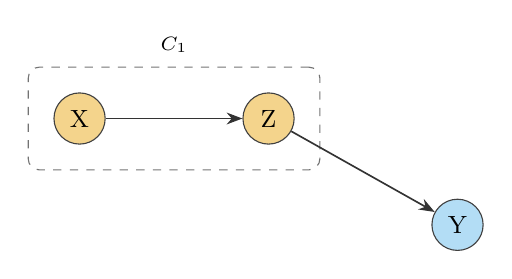
\begin{tikzpicture}
  \node[mannode] (nX) at (0.00,0.00) {X};
  \node[mannode] (nZ) at (2.40,0.00) {Z};
  \node[tgtnode] (nY) at (4.80,-1.35) {Y};
  \draw[diredge] (nX) -- (nZ);
  \draw[diredge] (nZ) -- (nY);
  \begin{scope}[on background layer]
    \node[clbox,fit=(nX)(nZ),label={[label distance=0.5mm]above:{\scriptsize$C_{1}$}}] {};
  \end{scope}
\end{tikzpicture}}\hfill
\adjustbox{max width=0.49\linewidth,valign=c}{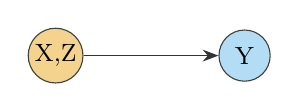
\begin{tikzpicture}
  \node[mannode] (nXZ) at (0.00,0.00) {X,Z};
  \node[tgtnode] (nY) at (2.40,0.00) {Y};
  \draw[diredge] (nXZ) -- (nY);
\end{tikzpicture}}
\caption{\textbf{ToyGraph.} Fine DAG with coarse partition (left) and quotient C-DAG (right), in the convention of Fig.~\ref{fig:clusterbench10}: manipulable variables orange, target blue, latent confounding dashed (intra-cluster) or dash-dotted (cross-cluster); dashed boxes are the manipulable clusters.}
\label{fig:dag-toyGraph}
\end{figure}

\begin{figure}[t]\centering
\adjustbox{max width=0.49\linewidth,valign=c}{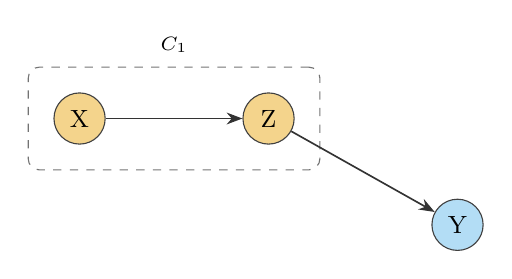
\begin{tikzpicture}
  \node[mannode] (nX) at (0.00,0.00) {X};
  \node[mannode] (nZ) at (2.40,0.00) {Z};
  \node[tgtnode] (nY) at (4.80,-1.35) {Y};
  \draw[diredge] (nX) -- (nZ);
  \draw[diredge] (nZ) -- (nY);
  \begin{scope}[on background layer]
    \node[clbox,fit=(nX)(nZ),label={[label distance=0.5mm]above:{\scriptsize$C_{1}$}}] {};
  \end{scope}
\end{tikzpicture}}\hfill
\adjustbox{max width=0.49\linewidth,valign=c}{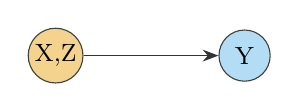
\begin{tikzpicture}
  \node[mannode] (nXZ) at (0.00,0.00) {X,Z};
  \node[tgtnode] (nY) at (2.40,0.00) {Y};
  \draw[diredge] (nXZ) -- (nY);
\end{tikzpicture}}
\caption{\textbf{Synthetic-2.} Fine DAG with coarse partition (left) and quotient C-DAG (right), in the convention of Fig.~\ref{fig:clusterbench10}: manipulable variables orange, target blue, latent confounding dashed (intra-cluster) or dash-dotted (cross-cluster); dashed boxes are the manipulable clusters.}
\label{fig:dag-synthetic_2}
\end{figure}

\begin{figure}[t]\centering
\adjustbox{max width=0.49\linewidth,valign=c}{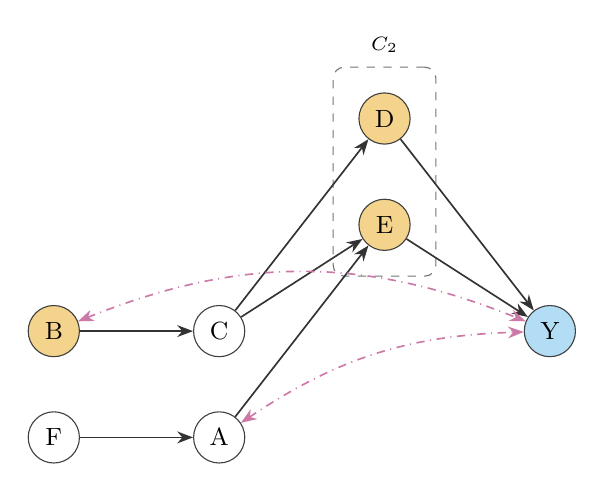
\begin{tikzpicture}
  \node[obsnode] (nF) at (0.00,-4.05) {F};
  \node[obsnode] (nA) at (2.10,-4.05) {A};
  \node[mannode] (nB) at (0.00,-2.70) {B};
  \node[obsnode] (nC) at (2.10,-2.70) {C};
  \node[mannode] (nD) at (4.20,0.00) {D};
  \node[mannode] (nE) at (4.20,-1.35) {E};
  \node[tgtnode] (nY) at (6.30,-2.70) {Y};
  \draw[diredge] (nF) -- (nA);
  \draw[diredge] (nB) -- (nC);
  \draw[diredge] (nC) -- (nD);
  \draw[diredge] (nA) -- (nE);
  \draw[diredge] (nC) -- (nE);
  \draw[diredge] (nD) -- (nY);
  \draw[diredge] (nE) -- (nY);
  \draw[bicross] (nA) to[bend left=16] (nY);
  \draw[bicross] (nB) to[bend left=22] (nY);
  \begin{scope}[on background layer]
    \node[clbox,fit=(nD)(nE),label={[label distance=0.5mm]above:{\scriptsize$C_{2}$}}] {};
  \end{scope}
\end{tikzpicture}}\hfill
\adjustbox{max width=0.49\linewidth,valign=c}{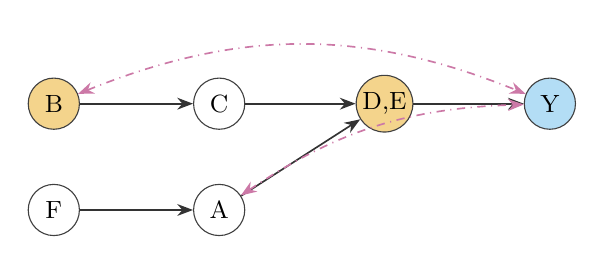
\begin{tikzpicture}
  \node[obsnode] (nF) at (0.00,-1.35) {F};
  \node[obsnode] (nA) at (2.10,-1.35) {A};
  \node[mannode] (nB) at (0.00,0.00) {B};
  \node[tgtnode] (nY) at (6.30,0.00) {Y};
  \node[mannode] (nDE) at (4.20,0.00) {D,E};
  \node[obsnode] (nC) at (2.10,0.00) {C};
  \draw[diredge] (nA) -- (nDE);
  \draw[diredge] (nB) -- (nC);
  \draw[diredge] (nDE) -- (nY);
  \draw[diredge] (nF) -- (nA);
  \draw[diredge] (nC) -- (nDE);
  \draw[bicross] (nA) to[bend left=16] (nY);
  \draw[bicross] (nB) to[bend left=22] (nY);
\end{tikzpicture}}
\caption{\textbf{Synthetic.} Fine DAG with coarse partition (left) and quotient C-DAG (right), in the convention of Fig.~\ref{fig:clusterbench10}: manipulable variables orange, target blue, latent confounding dashed (intra-cluster) or dash-dotted (cross-cluster); dashed boxes are the manipulable clusters.}
\label{fig:dag-synthetic}
\end{figure}

\begin{figure}[t]\centering
\adjustbox{max width=0.49\linewidth,valign=c}{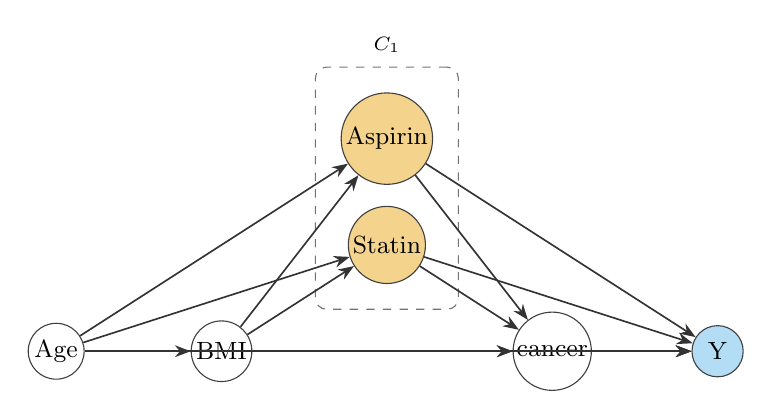
\begin{tikzpicture}
  \node[obsnode] (nAge) at (0.00,-2.70) {Age};
  \node[obsnode] (nBMI) at (2.10,-2.70) {BMI};
  \node[mannode] (nAspirin) at (4.20,0.00) {Aspirin};
  \node[mannode] (nStatin) at (4.20,-1.35) {Statin};
  \node[obsnode] (ncancer) at (6.30,-2.70) {cancer};
  \node[tgtnode] (nY) at (8.40,-2.70) {Y};
  \draw[diredge] (nAge) -- (nBMI);
  \draw[diredge] (nAge) -- (nAspirin);
  \draw[diredge] (nBMI) -- (nAspirin);
  \draw[diredge] (nAge) -- (nStatin);
  \draw[diredge] (nBMI) -- (nStatin);
  \draw[diredge] (nAge) -- (ncancer);
  \draw[diredge] (nBMI) -- (ncancer);
  \draw[diredge] (nStatin) -- (ncancer);
  \draw[diredge] (nAspirin) -- (ncancer);
  \draw[diredge] (nAge) -- (nY);
  \draw[diredge] (nBMI) -- (nY);
  \draw[diredge] (nStatin) -- (nY);
  \draw[diredge] (nAspirin) -- (nY);
  \draw[diredge] (ncancer) -- (nY);
  \begin{scope}[on background layer]
    \node[clbox,fit=(nAspirin)(nStatin),label={[label distance=0.5mm]above:{\scriptsize$C_{1}$}}] {};
  \end{scope}
\end{tikzpicture}}\hfill
\adjustbox{max width=0.49\linewidth,valign=c}{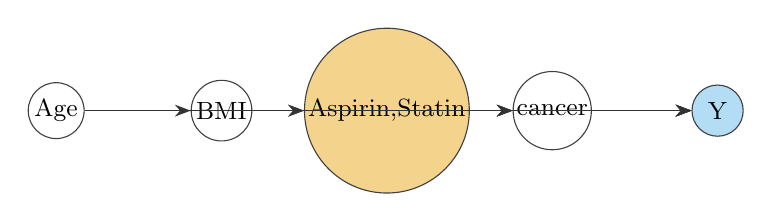
\begin{tikzpicture}
  \node[obsnode] (nAge) at (0.00,0.00) {Age};
  \node[mannode] (nAspirinStatin) at (4.20,0.00) {Aspirin,Statin};
  \node[obsnode] (nBMI) at (2.10,0.00) {BMI};
  \node[tgtnode] (nY) at (8.40,0.00) {Y};
  \node[obsnode] (ncancer) at (6.30,0.00) {cancer};
  \draw[diredge] (nBMI) -- (ncancer);
  \draw[diredge] (ncancer) -- (nY);
  \draw[diredge] (nBMI) -- (nY);
  \draw[diredge] (nAge) -- (ncancer);
  \draw[diredge] (nAspirinStatin) -- (ncancer);
  \draw[diredge] (nAge) -- (nY);
  \draw[diredge] (nBMI) -- (nAspirinStatin);
  \draw[diredge] (nAge) -- (nBMI);
  \draw[diredge] (nAspirinStatin) -- (nY);
  \draw[diredge] (nAge) -- (nAspirinStatin);
\end{tikzpicture}}
\caption{\textbf{Healthcare.} Fine DAG with coarse partition (left) and quotient C-DAG (right), in the convention of Fig.~\ref{fig:clusterbench10}: manipulable variables orange, target blue, latent confounding dashed (intra-cluster) or dash-dotted (cross-cluster); dashed boxes are the manipulable clusters.}
\label{fig:dag-healthcare}
\end{figure}

\begin{figure}[t]\centering
\adjustbox{max width=0.49\linewidth,valign=c}{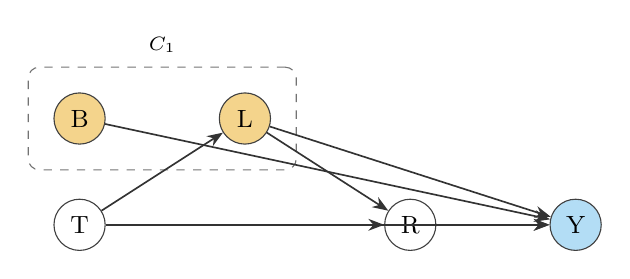
\begin{tikzpicture}
  \node[mannode] (nB) at (0.00,0.00) {B};
  \node[obsnode] (nT) at (0.00,-1.35) {T};
  \node[mannode] (nL) at (2.10,0.00) {L};
  \node[obsnode] (nR) at (4.20,-1.35) {R};
  \node[tgtnode] (nY) at (6.30,-1.35) {Y};
  \draw[diredge] (nT) -- (nL);
  \draw[diredge] (nL) -- (nR);
  \draw[diredge] (nT) -- (nR);
  \draw[diredge] (nT) -- (nY);
  \draw[diredge] (nL) -- (nY);
  \draw[diredge] (nR) -- (nY);
  \draw[diredge] (nB) -- (nY);
  \begin{scope}[on background layer]
    \node[clbox,fit=(nL)(nB),label={[label distance=0.5mm]above:{\scriptsize$C_{1}$}}] {};
  \end{scope}
\end{tikzpicture}}\hfill
\adjustbox{max width=0.49\linewidth,valign=c}{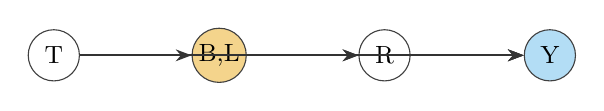
\begin{tikzpicture}
  \node[obsnode] (nT) at (0.00,0.00) {T};
  \node[mannode] (nBL) at (2.10,0.00) {B,L};
  \node[obsnode] (nR) at (4.20,0.00) {R};
  \node[tgtnode] (nY) at (6.30,0.00) {Y};
  \draw[diredge] (nR) -- (nY);
  \draw[diredge] (nT) -- (nBL);
  \draw[diredge] (nBL) -- (nR);
  \draw[diredge] (nT) -- (nR);
  \draw[diredge] (nBL) -- (nY);
  \draw[diredge] (nT) -- (nY);
\end{tikzpicture}}
\caption{\textbf{Epidemiology.} Fine DAG with coarse partition (left) and quotient C-DAG (right), in the convention of Fig.~\ref{fig:clusterbench10}: manipulable variables orange, target blue, latent confounding dashed (intra-cluster) or dash-dotted (cross-cluster); dashed boxes are the manipulable clusters.}
\label{fig:dag-epidemiology}
\end{figure}

\begin{figure}[t]\centering
\adjustbox{max width=0.49\linewidth,valign=c}{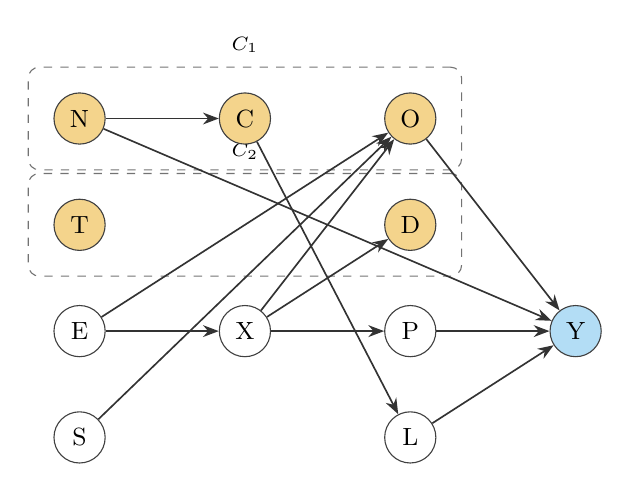
\begin{tikzpicture}
  \node[obsnode] (nE) at (0.00,-2.70) {E};
  \node[obsnode] (nS) at (0.00,-4.05) {S};
  \node[mannode] (nN) at (0.00,0.00) {N};
  \node[mannode] (nT) at (0.00,-1.35) {T};
  \node[obsnode] (nX) at (2.10,-2.70) {X};
  \node[mannode] (nC) at (2.10,0.00) {C};
  \node[obsnode] (nL) at (4.20,-4.05) {L};
  \node[obsnode] (nP) at (4.20,-2.70) {P};
  \node[mannode] (nD) at (4.20,-1.35) {D};
  \node[mannode] (nO) at (4.20,0.00) {O};
  \node[tgtnode] (nY) at (6.30,-2.70) {Y};
  \draw[diredge] (nE) -- (nX);
  \draw[diredge] (nN) -- (nC);
  \draw[diredge] (nC) -- (nL);
  \draw[diredge] (nX) -- (nP);
  \draw[diredge] (nX) -- (nD);
  \draw[diredge] (nE) -- (nO);
  \draw[diredge] (nS) -- (nO);
  \draw[diredge] (nX) -- (nO);
  \draw[diredge] (nL) -- (nY);
  \draw[diredge] (nN) -- (nY);
  \draw[diredge] (nP) -- (nY);
  \draw[diredge] (nO) -- (nY);
  \begin{scope}[on background layer]
    \node[clbox,fit=(nC)(nN)(nO),label={[label distance=0.5mm]above:{\scriptsize$C_{1}$}}] {};
  \end{scope}
  \begin{scope}[on background layer]
    \node[clbox,fit=(nD)(nT),label={[label distance=0.5mm]above:{\scriptsize$C_{2}$}}] {};
  \end{scope}
\end{tikzpicture}}\hfill
\adjustbox{max width=0.49\linewidth,valign=c}{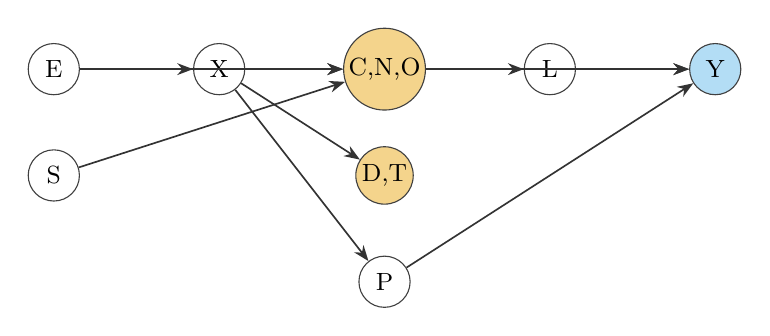
\begin{tikzpicture}
  \node[obsnode] (nL) at (6.30,0.00) {L};
  \node[obsnode] (nX) at (2.10,0.00) {X};
  \node[obsnode] (nS) at (0.00,-1.35) {S};
  \node[tgtnode] (nY) at (8.40,0.00) {Y};
  \node[mannode] (nDT) at (4.20,-1.35) {D,T};
  \node[mannode] (nCNO) at (4.20,0.00) {C,N,O};
  \node[obsnode] (nP) at (4.20,-2.70) {P};
  \node[obsnode] (nE) at (0.00,0.00) {E};
  \draw[diredge] (nCNO) -- (nL);
  \draw[diredge] (nE) -- (nCNO);
  \draw[diredge] (nS) -- (nCNO);
  \draw[diredge] (nL) -- (nY);
  \draw[diredge] (nCNO) -- (nY);
  \draw[diredge] (nX) -- (nDT);
  \draw[diredge] (nP) -- (nY);
  \draw[diredge] (nE) -- (nX);
  \draw[diredge] (nX) -- (nP);
  \draw[diredge] (nX) -- (nCNO);
\end{tikzpicture}}
\caption{\textbf{Ecology.} Fine DAG with coarse partition (left) and quotient C-DAG (right), in the convention of Fig.~\ref{fig:clusterbench10}: manipulable variables orange, target blue, latent confounding dashed (intra-cluster) or dash-dotted (cross-cluster); dashed boxes are the manipulable clusters.}
\label{fig:dag-ecology}
\end{figure}



\section{Full results}\label{app:fulltables}

\begin{figure}[!tb]\centering
  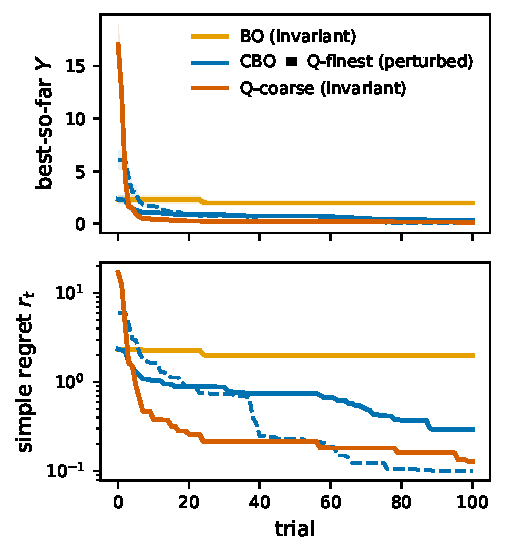
\includegraphics[width=\linewidth]{figures/clusterbench10_overlays}
  \caption{ClusterBench10: correct DAG (solid) vs intra-cluster bow $P_1$
  (dashed); bands are $\pm$\,s.e.\ over $10$ seeds. Top: best-so-far $Y$.
  Bottom: simple regret $r_t$ (log scale). \QCBO{}-coarse's and \BO{}'s
  dashed curves coincide exactly with their solid ones; the full-DAG pair's
  separate but both converge.}
  \label{fig:overlays}
\end{figure}

\begin{figure*}[t]\centering
  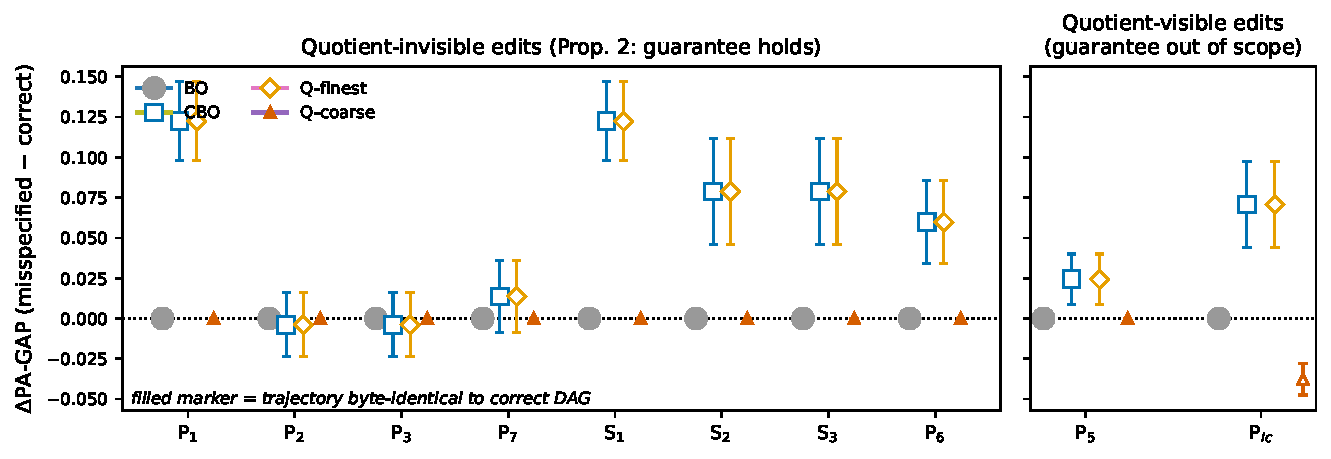
\includegraphics[width=\textwidth]{figures/clusterbench10_dial}
  \caption{$\Delta$PA-GAP (misspecified $-$ correct) for the whole
  perturbation field, split at the scope boundary of
  Prop.~\ref{prop:invariance}: quotient-\emph{invisible} edits (left) versus
  quotient-\emph{visible} (right). Filled markers: trajectories
  byte-identical to the correct-DAG run. \QCBO{}-coarse sits at exactly $0$
  across the left panel and departs only under the inter bow; the full-DAG
  method moves on every edge it can see.}
  \label{fig:dial}
\end{figure*}
Table~\ref{tab:fulltables} reports, for every method and every perturbation, the absolute
$\mathrm{GAP}$ at budgets $20/50/100$ and the paired degradation $\Delta\mathrm{GAP}@100$
and $\Delta\text{Final }Y$ (misspecified $-$ correct),
mean$\pm$s.e.\ over $10$ seeds at $T{=}100$. The \CBO{} and \QCBO{}-finest rows
coincide throughout, as they must by Prop.~\ref{prop:identity} (\CBO{} is
\QCBO{} at the finest partition $\Pi_\bot$). Table~\ref{tab:regret} reports the
corresponding regret: the simple regret $r_T$ of the final incumbent and the
cumulative regret $R_T$ of the incumbent sequence (\S\ref{sec:exp-setup}).
\begin{table}[t]\centering
\caption{ClusterBench10: full per-method, per-perturbation results
($10$ seeds, $T{=}100$). $\mathrm{GAP}\in[0,1]$, higher is more
sample-efficient; $\Delta$ columns are paired degradations versus the correct DAG, and
\textbf{b-id} marks byte-identical trajectories.}
\label{tab:fulltables}
\small\adjustbox{max width=\linewidth}{\begin{tabular}{@{}ll ccc cc c@{}}
\toprule
\textbf{Method} & \textbf{Pert.} & \textbf{GAP@20} & \textbf{GAP@50} & \textbf{GAP@100} & $\Delta$\textbf{GAP} & $\Delta Y_T$ & \textbf{ident.} \\
\midrule
\BO{} & P0 & $0.05{\scriptstyle\,\pm\,}0.05$ & $0.15{\scriptstyle\,\pm\,}0.08$ & $0.17{\scriptstyle\,\pm\,}0.09$ & -- & -- & \checkmark \\
 & P1 & $0.05{\scriptstyle\,\pm\,}0.05$ & $0.15{\scriptstyle\,\pm\,}0.08$ & $0.17{\scriptstyle\,\pm\,}0.09$ & $+0.000{\scriptstyle\,\pm\,}0.000$ & $+0.000{\scriptstyle\,\pm\,}0.000$ & \checkmark \\
 & P2 & $0.05{\scriptstyle\,\pm\,}0.05$ & $0.15{\scriptstyle\,\pm\,}0.08$ & $0.17{\scriptstyle\,\pm\,}0.09$ & $+0.000{\scriptstyle\,\pm\,}0.000$ & $+0.000{\scriptstyle\,\pm\,}0.000$ & \checkmark \\
 & P3 & $0.05{\scriptstyle\,\pm\,}0.05$ & $0.15{\scriptstyle\,\pm\,}0.08$ & $0.17{\scriptstyle\,\pm\,}0.09$ & $+0.000{\scriptstyle\,\pm\,}0.000$ & $+0.000{\scriptstyle\,\pm\,}0.000$ & \checkmark \\
 & P7 & $0.05{\scriptstyle\,\pm\,}0.05$ & $0.15{\scriptstyle\,\pm\,}0.08$ & $0.17{\scriptstyle\,\pm\,}0.09$ & $+0.000{\scriptstyle\,\pm\,}0.000$ & $+0.000{\scriptstyle\,\pm\,}0.000$ & \checkmark \\
 & S1 & $0.05{\scriptstyle\,\pm\,}0.05$ & $0.15{\scriptstyle\,\pm\,}0.08$ & $0.17{\scriptstyle\,\pm\,}0.09$ & $+0.000{\scriptstyle\,\pm\,}0.000$ & $+0.000{\scriptstyle\,\pm\,}0.000$ & \checkmark \\
 & S2 & $0.05{\scriptstyle\,\pm\,}0.05$ & $0.15{\scriptstyle\,\pm\,}0.08$ & $0.17{\scriptstyle\,\pm\,}0.09$ & $+0.000{\scriptstyle\,\pm\,}0.000$ & $+0.000{\scriptstyle\,\pm\,}0.000$ & \checkmark \\
 & S3 & $0.05{\scriptstyle\,\pm\,}0.05$ & $0.15{\scriptstyle\,\pm\,}0.08$ & $0.17{\scriptstyle\,\pm\,}0.09$ & $+0.000{\scriptstyle\,\pm\,}0.000$ & $+0.000{\scriptstyle\,\pm\,}0.000$ & \checkmark \\
 & P6 & $0.05{\scriptstyle\,\pm\,}0.05$ & $0.15{\scriptstyle\,\pm\,}0.08$ & $0.17{\scriptstyle\,\pm\,}0.09$ & $+0.000{\scriptstyle\,\pm\,}0.000$ & $+0.000{\scriptstyle\,\pm\,}0.000$ & \checkmark \\
 & P5 & $0.05{\scriptstyle\,\pm\,}0.05$ & $0.15{\scriptstyle\,\pm\,}0.08$ & $0.17{\scriptstyle\,\pm\,}0.09$ & $+0.000{\scriptstyle\,\pm\,}0.000$ & $+0.000{\scriptstyle\,\pm\,}0.000$ & \checkmark \\
 & Pic & $0.05{\scriptstyle\,\pm\,}0.05$ & $0.15{\scriptstyle\,\pm\,}0.08$ & $0.17{\scriptstyle\,\pm\,}0.09$ & $+0.000{\scriptstyle\,\pm\,}0.000$ & $+0.000{\scriptstyle\,\pm\,}0.000$ & \checkmark \\
\midrule
\CBO{} & P0 & $0.46{\scriptstyle\,\pm\,}0.06$ & $0.52{\scriptstyle\,\pm\,}0.07$ & $0.56{\scriptstyle\,\pm\,}0.03$ & -- & -- & \checkmark \\
 & P1 & $0.57{\scriptstyle\,\pm\,}0.05$ & $0.63{\scriptstyle\,\pm\,}0.03$ & $0.68{\scriptstyle\,\pm\,}0.03$ & $+0.116{\scriptstyle\,\pm\,}0.043$ & $-0.190{\scriptstyle\,\pm\,}0.052$ & -- \\
 & P2 & $0.28{\scriptstyle\,\pm\,}0.07$ & $0.58{\scriptstyle\,\pm\,}0.05$ & $0.72{\scriptstyle\,\pm\,}0.04$ & $+0.156{\scriptstyle\,\pm\,}0.039$ & $-0.157{\scriptstyle\,\pm\,}0.052$ & -- \\
 & P3 & $0.28{\scriptstyle\,\pm\,}0.07$ & $0.58{\scriptstyle\,\pm\,}0.05$ & $0.72{\scriptstyle\,\pm\,}0.04$ & $+0.156{\scriptstyle\,\pm\,}0.039$ & $-0.157{\scriptstyle\,\pm\,}0.052$ & -- \\
 & P7 & $0.33{\scriptstyle\,\pm\,}0.06$ & $0.57{\scriptstyle\,\pm\,}0.03$ & $0.66{\scriptstyle\,\pm\,}0.05$ & $+0.098{\scriptstyle\,\pm\,}0.038$ & $-0.171{\scriptstyle\,\pm\,}0.039$ & -- \\
 & S1 & $0.57{\scriptstyle\,\pm\,}0.05$ & $0.63{\scriptstyle\,\pm\,}0.03$ & $0.68{\scriptstyle\,\pm\,}0.03$ & $+0.116{\scriptstyle\,\pm\,}0.043$ & $-0.190{\scriptstyle\,\pm\,}0.052$ & -- \\
 & S2 & $0.53{\scriptstyle\,\pm\,}0.05$ & $0.58{\scriptstyle\,\pm\,}0.04$ & $0.68{\scriptstyle\,\pm\,}0.03$ & $+0.120{\scriptstyle\,\pm\,}0.049$ & $-0.182{\scriptstyle\,\pm\,}0.055$ & -- \\
 & S3 & $0.53{\scriptstyle\,\pm\,}0.05$ & $0.58{\scriptstyle\,\pm\,}0.04$ & $0.68{\scriptstyle\,\pm\,}0.03$ & $+0.120{\scriptstyle\,\pm\,}0.049$ & $-0.181{\scriptstyle\,\pm\,}0.055$ & -- \\
 & P6 & $0.43{\scriptstyle\,\pm\,}0.04$ & $0.62{\scriptstyle\,\pm\,}0.03$ & $0.68{\scriptstyle\,\pm\,}0.04$ & $+0.122{\scriptstyle\,\pm\,}0.052$ & $-0.198{\scriptstyle\,\pm\,}0.048$ & -- \\
 & P5 & $0.46{\scriptstyle\,\pm\,}0.05$ & $0.56{\scriptstyle\,\pm\,}0.05$ & $0.60{\scriptstyle\,\pm\,}0.04$ & $+0.040{\scriptstyle\,\pm\,}0.032$ & $-0.091{\scriptstyle\,\pm\,}0.043$ & -- \\
 & Pic & $0.47{\scriptstyle\,\pm\,}0.03$ & $0.54{\scriptstyle\,\pm\,}0.04$ & $0.57{\scriptstyle\,\pm\,}0.03$ & $+0.007{\scriptstyle\,\pm\,}0.035$ & $+0.070{\scriptstyle\,\pm\,}0.073$ & -- \\
\midrule
\QCBO{} & P0 & $0.73{\scriptstyle\,\pm\,}0.05$ & $0.89{\scriptstyle\,\pm\,}0.02$ & $0.77{\scriptstyle\,\pm\,}0.07$ & -- & -- & \checkmark \\
 & P1 & $0.73{\scriptstyle\,\pm\,}0.05$ & $0.89{\scriptstyle\,\pm\,}0.02$ & $0.77{\scriptstyle\,\pm\,}0.07$ & $+0.000{\scriptstyle\,\pm\,}0.000$ & $+0.000{\scriptstyle\,\pm\,}0.000$ & \checkmark \\
 & P2 & $0.73{\scriptstyle\,\pm\,}0.05$ & $0.89{\scriptstyle\,\pm\,}0.02$ & $0.77{\scriptstyle\,\pm\,}0.07$ & $+0.000{\scriptstyle\,\pm\,}0.000$ & $+0.000{\scriptstyle\,\pm\,}0.000$ & \checkmark \\
 & P3 & $0.73{\scriptstyle\,\pm\,}0.05$ & $0.89{\scriptstyle\,\pm\,}0.02$ & $0.77{\scriptstyle\,\pm\,}0.07$ & $+0.000{\scriptstyle\,\pm\,}0.000$ & $+0.000{\scriptstyle\,\pm\,}0.000$ & \checkmark \\
 & P7 & $0.73{\scriptstyle\,\pm\,}0.05$ & $0.89{\scriptstyle\,\pm\,}0.02$ & $0.77{\scriptstyle\,\pm\,}0.07$ & $+0.000{\scriptstyle\,\pm\,}0.000$ & $+0.000{\scriptstyle\,\pm\,}0.000$ & \checkmark \\
 & S1 & $0.73{\scriptstyle\,\pm\,}0.05$ & $0.89{\scriptstyle\,\pm\,}0.02$ & $0.77{\scriptstyle\,\pm\,}0.07$ & $+0.000{\scriptstyle\,\pm\,}0.000$ & $+0.000{\scriptstyle\,\pm\,}0.000$ & \checkmark \\
 & S2 & $0.73{\scriptstyle\,\pm\,}0.05$ & $0.89{\scriptstyle\,\pm\,}0.02$ & $0.77{\scriptstyle\,\pm\,}0.07$ & $+0.000{\scriptstyle\,\pm\,}0.000$ & $+0.000{\scriptstyle\,\pm\,}0.000$ & \checkmark \\
 & S3 & $0.73{\scriptstyle\,\pm\,}0.05$ & $0.89{\scriptstyle\,\pm\,}0.02$ & $0.77{\scriptstyle\,\pm\,}0.07$ & $+0.000{\scriptstyle\,\pm\,}0.000$ & $+0.000{\scriptstyle\,\pm\,}0.000$ & \checkmark \\
 & P6 & $0.73{\scriptstyle\,\pm\,}0.05$ & $0.89{\scriptstyle\,\pm\,}0.02$ & $0.77{\scriptstyle\,\pm\,}0.07$ & $+0.000{\scriptstyle\,\pm\,}0.000$ & $+0.000{\scriptstyle\,\pm\,}0.000$ & \checkmark \\
 & P5 & $0.73{\scriptstyle\,\pm\,}0.05$ & $0.89{\scriptstyle\,\pm\,}0.02$ & $0.77{\scriptstyle\,\pm\,}0.07$ & $+0.000{\scriptstyle\,\pm\,}0.000$ & $+0.000{\scriptstyle\,\pm\,}0.000$ & \checkmark \\
 & Pic & $0.70{\scriptstyle\,\pm\,}0.04$ & $0.73{\scriptstyle\,\pm\,}0.05$ & $0.76{\scriptstyle\,\pm\,}0.05$ & $-0.007{\scriptstyle\,\pm\,}0.084$ & $+0.538{\scriptstyle\,\pm\,}0.085$ & -- \\
\bottomrule
\end{tabular}
}
\end{table}
\begin{table}[t]\centering
\caption{ClusterBench10: simple regret $r_T$ ($\downarrow$) and cumulative
incumbent regret $R_T$ ($\downarrow$) per method and perturbation
($10$ seeds, $T{=}100$; $y^\star{=}0$).}
\label{tab:regret}
\small\adjustbox{max width=\linewidth}{\begin{tabular}{@{}lcccccc@{}}
\toprule
\textbf{Pert.} & \multicolumn{2}{c}{\textbf{\BO{}}} & \multicolumn{2}{c}{\textbf{\CBO{}}} & \multicolumn{2}{c}{\textbf{\QCBO{}}} \\
\cmidrule(lr){2-3}\cmidrule(lr){4-5}\cmidrule(lr){6-7}
 & $r_T$ & $R_T$ & $r_T$ & $R_T$ & $r_T$ & $R_T$ \\
\midrule
P0 & $1.98{\scriptstyle\,\pm\,}0.26$ & $205.6{\scriptstyle\,\pm\,}27.1$ & $0.29{\scriptstyle\,\pm\,}0.05$ & $71.3{\scriptstyle\,\pm\,}5.6$ & $0.13{\scriptstyle\,\pm\,}0.02$ & $41.8{\scriptstyle\,\pm\,}5.2$ \\
P1 & $1.98{\scriptstyle\,\pm\,}0.26$ & $205.6{\scriptstyle\,\pm\,}27.1$ & $0.10{\scriptstyle\,\pm\,}0.02$ & $65.8{\scriptstyle\,\pm\,}4.6$ & $0.13{\scriptstyle\,\pm\,}0.02$ & $41.8{\scriptstyle\,\pm\,}5.2$ \\
P2 & $1.98{\scriptstyle\,\pm\,}0.26$ & $205.6{\scriptstyle\,\pm\,}27.1$ & $0.13{\scriptstyle\,\pm\,}0.03$ & $62.3{\scriptstyle\,\pm\,}5.4$ & $0.13{\scriptstyle\,\pm\,}0.02$ & $41.8{\scriptstyle\,\pm\,}5.2$ \\
P3 & $1.98{\scriptstyle\,\pm\,}0.26$ & $205.6{\scriptstyle\,\pm\,}27.1$ & $0.13{\scriptstyle\,\pm\,}0.03$ & $62.3{\scriptstyle\,\pm\,}5.4$ & $0.13{\scriptstyle\,\pm\,}0.02$ & $41.8{\scriptstyle\,\pm\,}5.2$ \\
P7 & $1.98{\scriptstyle\,\pm\,}0.26$ & $205.6{\scriptstyle\,\pm\,}27.1$ & $0.12{\scriptstyle\,\pm\,}0.03$ & $58.1{\scriptstyle\,\pm\,}5.5$ & $0.13{\scriptstyle\,\pm\,}0.02$ & $41.8{\scriptstyle\,\pm\,}5.2$ \\
S1 & $1.98{\scriptstyle\,\pm\,}0.26$ & $205.6{\scriptstyle\,\pm\,}27.1$ & $0.10{\scriptstyle\,\pm\,}0.02$ & $65.8{\scriptstyle\,\pm\,}4.6$ & $0.13{\scriptstyle\,\pm\,}0.02$ & $41.8{\scriptstyle\,\pm\,}5.2$ \\
S2 & $1.98{\scriptstyle\,\pm\,}0.26$ & $205.6{\scriptstyle\,\pm\,}27.1$ & $0.11{\scriptstyle\,\pm\,}0.03$ & $98.1{\scriptstyle\,\pm\,}11.6$ & $0.13{\scriptstyle\,\pm\,}0.02$ & $41.8{\scriptstyle\,\pm\,}5.2$ \\
S3 & $1.98{\scriptstyle\,\pm\,}0.26$ & $205.6{\scriptstyle\,\pm\,}27.1$ & $0.11{\scriptstyle\,\pm\,}0.03$ & $98.0{\scriptstyle\,\pm\,}11.6$ & $0.13{\scriptstyle\,\pm\,}0.02$ & $41.8{\scriptstyle\,\pm\,}5.2$ \\
P6 & $1.98{\scriptstyle\,\pm\,}0.26$ & $205.6{\scriptstyle\,\pm\,}27.1$ & $0.09{\scriptstyle\,\pm\,}0.02$ & $43.9{\scriptstyle\,\pm\,}3.9$ & $0.13{\scriptstyle\,\pm\,}0.02$ & $41.8{\scriptstyle\,\pm\,}5.2$ \\
P5 & $1.98{\scriptstyle\,\pm\,}0.26$ & $205.6{\scriptstyle\,\pm\,}27.1$ & $0.20{\scriptstyle\,\pm\,}0.05$ & $59.0{\scriptstyle\,\pm\,}6.4$ & $0.13{\scriptstyle\,\pm\,}0.02$ & $41.8{\scriptstyle\,\pm\,}5.2$ \\
Pic & $1.98{\scriptstyle\,\pm\,}0.26$ & $205.6{\scriptstyle\,\pm\,}27.1$ & $0.36{\scriptstyle\,\pm\,}0.08$ & $93.2{\scriptstyle\,\pm\,}4.5$ & $0.67{\scriptstyle\,\pm\,}0.07$ & $99.6{\scriptstyle\,\pm\,}4.0$ \\
\bottomrule
\end{tabular}
}
\end{table}

\section{The cost of a wrong partition}\label{app:wrongpi}
\QCBO{} consumes only the C-DAG and never the fine graph, so a wrong
\emph{partition} is stressed by quotienting the base structure once under
$\{X_1,X_2,X_4\},\{X_3,X_5\}$ ($X_3$ and $X_4$ swapped) to obtain a fixed,
acyclic but incorrect C-DAG, and optimizing the true objective through it.
The wrong partition alters the exploration set, identification verdicts, and
priors, but not the objective; by construction it is invariant to the
fine-structure perturbations of \S\ref{sec:exp-scope}, so it has a single
cost, reported in Table~\ref{tab:wrongpi}: final quality degrades
($Y=0.49$ vs $0.13$ correct-partition, $0.29$ \CBO{}) while GAP and PA-GAP
stay within $0.06$ of the correct coarse run and \BO{}.

\begin{table}[h]\centering
  \caption{Cost of a \emph{wrong} partition on \textsc{ClusterBench10} (correct
  objective; 10 seeds, $T{=}100$, $y^\star{=}0$). \QCBO{}-wrong$\Pi$ holds a fixed,
  acyclic but incorrect C-DAG (base structure under a wrong partition). It loses
  final quality against the correct partition yet degrades gracefully, staying far
  above non-causal \BO{}.}
  \label{tab:wrongpi}
  \small
  \adjustbox{max width=\linewidth}{\begin{tabular}{@{}lccc@{}}
\toprule
\textbf{Method} & \textbf{Final $Y$} & $r_T$ & \textbf{GAP@100} \\
\multicolumn{1}{c}{} & \multicolumn{2}{c}{\footnotesize $\downarrow$, $y^\star{=}0$} & {\footnotesize $\uparrow$ secondary} \\
\midrule
\BO & $1.981{\scriptstyle\,\pm\,}0.261$ & $1.981{\scriptstyle\,\pm\,}0.261$ & $0.175{\scriptstyle\,\pm\,}0.090$ \\
\CBO & $0.290{\scriptstyle\,\pm\,}0.054$ & $0.290{\scriptstyle\,\pm\,}0.054$ & $0.561{\scriptstyle\,\pm\,}0.033$ \\
\textbf{\QCBO{}}\;{\footnotesize(correct $\Pi$)} & $0.128{\scriptstyle\,\pm\,}0.021$ & $0.128{\scriptstyle\,\pm\,}0.021$ & $0.769{\scriptstyle\,\pm\,}0.066$ \\
\QCBO{}-wrong$\Pi$\;{\footnotesize(wrong $\Pi$)} & $0.491{\scriptstyle\,\pm\,}0.088$ & $0.491{\scriptstyle\,\pm\,}0.088$ & $0.714{\scriptstyle\,\pm\,}0.037$ \\
\bottomrule
\end{tabular}
}
\end{table}

\section{\QCBO{}-refine across datasets}\label{app:refine}

\begin{figure}[t]\centering
  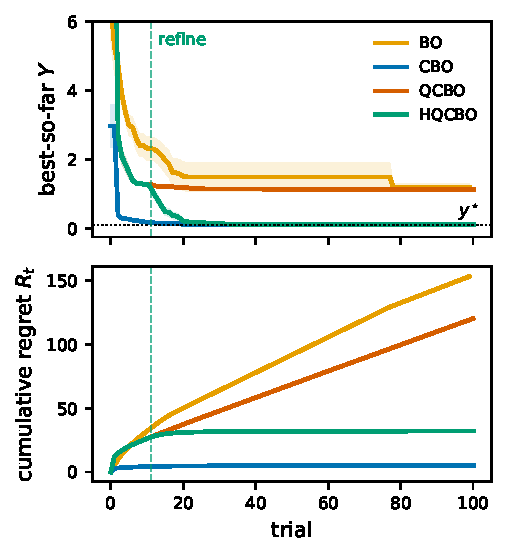
\includegraphics[width=\linewidth]{figures/clusterbench10L_refine}
  \caption{\QCBO{}-refine on \textsc{ClusterBench10L} (10 seeds, mean
  $\pm$ s.e.; dashed vertical line = mean trigger). Top: best-so-far $Y$ ---
  refine rides the coarse trajectory, then splits $C_1$ and descends to
  $y^\star$. Bottom: cumulative incumbent regret $R_t$ --- fixed-coarse is
  linear in $t$, refine's flattens after the trigger
  (Remark~\ref{rem:regret}).}
  \label{fig:refine}
\end{figure}

Table~\ref{tab:refine-suite} and Fig.~\ref{fig:refine-suite} give the full
cross-dataset picture for \QCBO{}-refine (\S\ref{sec:refine}): the two
\textsc{ClusterBench} variants and the three survey datasets whose domain
partition we refine ($10$ seeds on the \textsc{ClusterBench} pair, $5$ on the
survey datasets; the finest run supplies the \CBO{} row by
Prop.~\ref{prop:identity}). Three regimes are visible. \emph{(i) Lossless,
partition helps} (\textsc{ClusterBench10}): both quotient methods beat \CBO{}
on final $Y$ and cumulative regret, and refinement adds a little more; the
false trigger --- refine cannot observe $y^\star$, so it fires anyway --- costs
nothing ($R_T\,41.6$ vs coarse $41.8$). \emph{(ii) Lossy}
(\textsc{ClusterBench10L}, \textsc{synthetic\_2}): fixed-coarse plateaus and
its cumulative regret grows linearly; refinement escapes the plateau to
\CBO{}'s optimum ($-1.855$ vs finest $-2.054$ on \textsc{synthetic\_2}) and
bends $R_T$ back toward the better of \{coarse, \CBO{}\}. \emph{(iii) Lossless,
partition neutral} (\textsc{ecology}, \textsc{healthcare}): the four methods
sit within noise on final $Y$; here the false trigger costs a small polish tax
on \textsc{ecology} ($4.885$ vs coarse $4.983$, task max) and nothing
measurable on \textsc{healthcare}. Two honest reads follow. Refinement lowers
GAP relative to fixed-coarse everywhere --- the mid-run split adds arms and
re-explores, trading early-budget GAP for the final-value and regret recovery
--- so it is the right default only when the partition is suspected lossy.
And on the small survey partitions ($2$--$5$ manipulable variables) neither
quotient method dominates full-knowledge \CBO{} on final $Y$; the clear wins
are on the constructed benchmarks, where the cluster count is large enough for
coarsening's focus to register. This is the finite-budget, few-cluster regime;
the $\Theta(K^m)$-vs-$\Theta(N^m)$ arm-count gap that motivates coarsening
widens with problem size, which these $N\!\le\!10$ datasets do not exercise.

\begin{table}[t]\centering
\caption{\QCBO{}-refine vs \BO{}, \CBO{}, and \QCBO{}-coarse across datasets.
Final $Y$ (closest to $y^\star$ best), GAP@100 ($\uparrow$), cumulative
incumbent regret $R_T$ ($\downarrow$); mean$\pm$s.e., best per group in bold.}
\label{tab:refine-suite}
\small\adjustbox{max width=\linewidth}{\begin{tabular}{@{}llccc@{}}
\toprule
\textbf{Dataset} & \textbf{Method} & \textbf{Final $Y$} & \textbf{GAP@100} & $R_T$ \\
 & & {\footnotesize $\to y^\star$} & {\footnotesize $\uparrow$} & {\footnotesize $\downarrow$} \\
\midrule
\multicolumn{5}{@{}l}{\emph{\textsc{ClusterBench10}} {\footnotesize(lossless, $y^\star{=}0$)}} \\
\quad & \BO & $1.981{\scriptstyle\,\pm\,}0.261$ & $0.175{\scriptstyle\,\pm\,}0.090$ & $205.6{\scriptstyle\,\pm\,}27.1$ \\
\quad & \CBO & $0.290{\scriptstyle\,\pm\,}0.054$ & $0.561{\scriptstyle\,\pm\,}0.033$ & $71.3{\scriptstyle\,\pm\,}5.6$ \\
\quad & \QCBO{} & $0.128{\scriptstyle\,\pm\,}0.021$ & $\mathbf{0.769{\scriptstyle\,\pm\,}0.066}$ & $41.8{\scriptstyle\,\pm\,}5.2$ \\
\quad & \textbf{\HQCBO{}} & $\mathbf{0.070{\scriptstyle\,\pm\,}0.021}$ & $0.704{\scriptstyle\,\pm\,}0.059$ & $\mathbf{41.6{\scriptstyle\,\pm\,}5.8}$ \\
\addlinespace[2pt]
\multicolumn{5}{@{}l}{\emph{\textsc{ClusterBench10L}} {\footnotesize(lossy, $y^\star{=}0.10$)}} \\
\quad & \BO & $1.188{\scriptstyle\,\pm\,}0.122$ & $0.765{\scriptstyle\,\pm\,}0.044$ & $153.3{\scriptstyle\,\pm\,}32.6$ \\
\quad & \QCBO{} & $1.128{\scriptstyle\,\pm\,}0.016$ & $\mathbf{0.802{\scriptstyle\,\pm\,}0.036}$ & $120.3{\scriptstyle\,\pm\,}3.1$ \\
\quad & \textbf{\HQCBO{}} & $\mathbf{0.101{\scriptstyle\,\pm\,}0.001}$ & $0.694{\scriptstyle\,\pm\,}0.037$ & $\mathbf{32.1{\scriptstyle\,\pm\,}2.6}$ \\
\bottomrule
\end{tabular}
}
\end{table}

\begin{figure}[t]\centering
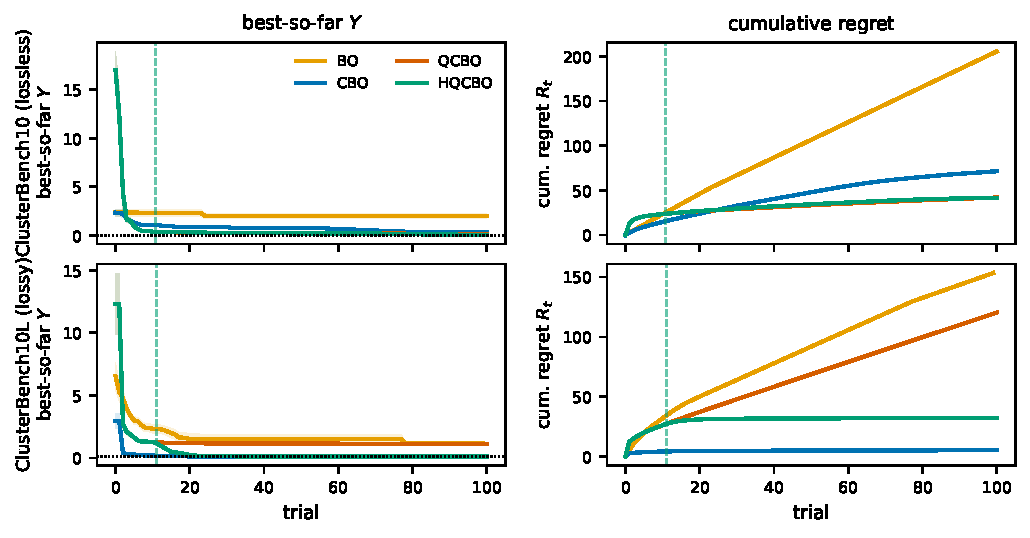
\includegraphics[width=0.86\linewidth]{figures/refine_suite}
\caption{Best-so-far $Y$ (left) and cumulative incumbent regret $R_t$ (right)
per dataset; mean $\pm$ s.e., dashed line = mean \QCBO{}-refine trigger.
\CBO{}$\,\equiv\,$\QCBO{}-finest (Prop.~\ref{prop:identity}). Refinement rides
coarse until the trigger, then --- where the partition is lossy
(\textsc{ClusterBench10L}, \textsc{synthetic\_2}) --- descends and flattens
$R_t$; where it is lossless the trajectories stay together.}
\label{fig:refine-suite}
\end{figure}

% =============================================================================
\bibliographystyle{abbrvnat}
\begin{thebibliography}{27}

\bibitem[Aglietti et al.(2020)]{aglietti2020causal}
V.~Aglietti, X.~Lu, A.~Paleyes, and J.~Gonz{\'a}lez.
\newblock Causal {B}ayesian optimization.
\newblock In \emph{AISTATS}, volume 108 of \emph{PMLR}, pp.\ 3155--3164, 2020.

\bibitem[Aglietti et al.(2021)]{aglietti2021dynamic}
V.~Aglietti, N.~Dhir, J.~Gonz{\'a}lez, and T.~Damoulas.
\newblock Dynamic causal {B}ayesian optimization.
\newblock In \emph{NeurIPS}, volume 34, 2021.

\bibitem[Aglietti et al.(2023)]{aglietti2023constrained}
V.~Aglietti, A.~Malek, I.~Ktena, and S.~Chiappa.
\newblock Constrained causal {B}ayesian optimization.
\newblock In \emph{ICML}, 2023.

\bibitem[Anand et al.(2023)]{anand2023cdag}
T.~V.~Anand, A.~H.~Ribeiro, J.~Tian, and E.~Bareinboim.
\newblock Causal effect identification in cluster {DAG}s.
\newblock In \emph{AAAI}, volume 37, pp.\ 12172--12179, 2023.

\bibitem[Anonymous(2026)]{anonymous2026cbobench}
Anonymous.
\newblock Causal {B}ayesian optimization: Foundations, methods, and applications.
\newblock \emph{Transactions on Machine Learning Research}, 2026.
\newblock Under review; OpenReview \url{https://openreview.net/forum?id=XT6DC37m5I}.

\bibitem[Arsenyan et al.(2026)]{arsenyan2026contextual}
V.~Arsenyan, A.~Grosnit, H.~Bou~Ammar, and A.~Dalalyan.
\newblock Contextual causal {B}ayesian optimisation.
\newblock In \emph{ICLR}, 2026.

\bibitem[Beckers \& Halpern(2019)]{beckers2019approximate}
S.~Beckers and J.~Y.~Halpern.
\newblock Abstracting causal models.
\newblock In \emph{AAAI}, 2019.

\bibitem[Branchini et al.(2023)]{branchini2023ceo}
N.~Branchini, V.~Aglietti, N.~Dhir, and T.~Damoulas.
\newblock Causal entropy optimization.
\newblock In \emph{AISTATS}, volume 206 of \emph{PMLR}, pp.\ 8586--8605, 2023.

\bibitem[Durand et al.(2025)]{durand2025unknown}
J.~Durand, Y.~Annadani, S.~Bauer, and S.~Parbhoo.
\newblock Causal {B}ayesian optimization with unknown graphs.
\newblock \emph{arXiv:2503.19554}, 2025.

\bibitem[Ferreira \& Assaad(2025)]{ferreira2025cdmg}
E.~Ferreira and C.~K.~Assaad.
\newblock Identifying macro causal effects in a {C-DMG} over {ADMG}s.
\newblock \emph{arXiv:2504.01551}, 2025.

\bibitem[Garnett(2023)]{garnett2023bayesian}
R.~Garnett.
\newblock \emph{Bayesian Optimization}.
\newblock Cambridge University Press, 2023.

\bibitem[Lee et al.(2023)]{lee2023ananke}
J.~J.~R.~Lee, R.~Bhattacharya, R.~Nabi, and I.~Shpitser.
\newblock Ananke: A python package for causal inference using graphical models.
\newblock \emph{arXiv:2301.11477}, 2023.

\bibitem[Lee \& Bareinboim(2018)]{lee2018structural}
S.~Lee and E.~Bareinboim.
\newblock Structural causal bandits: Where to intervene?
\newblock In \emph{NeurIPS}, 2018.

\bibitem[Lee et al.(2019)]{lee2019latent}
S.~Lee, J.~Correa, and E.~Bareinboim.
\newblock General identifiability with arbitrary surrogate experiments.
\newblock In \emph{UAI}, 2019.

\bibitem[Madaleno et al.(2026a)]{madaleno2026coarsening}
F.~Madaleno, P.~Misra, and A.~Markham.
\newblock Coarsening causal {DAG} models.
\newblock \emph{arXiv:2601.10531}, 2026a.

\bibitem[Madaleno et al.(2026b)]{madaleno2026cycles}
F.~Madaleno, F.~C.~Pereira, and A.~Markham.
\newblock Coarsening linear non-{G}aussian causal models with cycles.
\newblock \emph{arXiv:2605.10163}, 2026b.

\bibitem[Mukherjee et al.(2024)]{mukherjee2024gacbo}
S.~Mukherjee, M.~Zhang, S.~Flaxman, and S.~J.~Vollmer.
\newblock Graph agnostic causal {B}ayesian optimisation.
\newblock \emph{arXiv:2411.03028}, 2024.

\bibitem[Park et al.(2025)]{park2025dmis}
J.~Park, M.~Zemplenyi, and V.~Aglietti.
\newblock Causal {B}ayesian optimization under partial observability.
\newblock \emph{arXiv}, 2025.

\bibitem[Pearl(2009)]{pearl2009causality}
J.~Pearl.
\newblock \emph{Causality: Models, Reasoning and Inference}.
\newblock Cambridge University Press, 2nd edition, 2009.

\bibitem[Poloczek et al.(2017)]{poloczek2017multi}
M.~Poloczek, J.~Wang, and P.~Frazier.
\newblock Multi-information source optimization.
\newblock In \emph{NeurIPS}, 2017.

\bibitem[Ruiz~de~Vargas et al.(2025)]{ruizdevargas2025cdags}
J.~M.~Ruiz~de~Vargas, K.~Padh, and N.~Kilbertus.
\newblock Cluster-{DAG}s as powerful background knowledge for causal discovery.
\newblock \emph{arXiv:2512.10032}, 2025.

\bibitem[Shpitser \& Pearl(2006)]{shpitser2006identification}
I.~Shpitser and J.~Pearl.
\newblock Identification of joint interventional distributions in recursive
semi-{M}arkovian causal models.
\newblock In \emph{AAAI}, 2006.

\bibitem[Sussex et al.(2023)]{sussex2023model}
S.~Sussex, A.~Makarova, and A.~Krause.
\newblock Model-based causal {B}ayesian optimization.
\newblock In \emph{ICLR}, 2023.

\bibitem[Wahl et al.(2024)]{wahl2024foundations}
J.~Wahl, U.~Ninad, and J.~Runge.
\newblock Foundations of causal discovery on groups of variables.
\newblock \emph{Journal of Causal Inference}, 12(1), 2024.

\bibitem[Yvernes et al.(2025)]{yvernes2025relaxing}
C.~Yvernes, E.~Devijver, A.~H.~Ribeiro, M.~Clausel-Lesourd, and \'E.~Gaussier.
\newblock Relaxing partition admissibility in cluster-{DAG}s: a causal calculus
with arbitrary variable clustering.
\newblock \emph{arXiv:2511.01396}, 2025.

\bibitem[Zeitler(2025)]{zeitler2025mfacbo}
J.~Zeitler.
\newblock Towards {MFACBO}: Multi-fidelity abstraction causal {B}ayesian
optimization.
\newblock In \emph{Workshop on Causal Abstractions and Representations (CAR) at UAI}, 2025.

\end{thebibliography}

\end{document}